\documentclass[12pt,a4paper,oneside]{report}

% ---------------------------------------------------------
% Essential Packages
% ---------------------------------------------------------
\usepackage[utf8]{inputenc}
\usepackage[margin=1in, left=1.25in, top=1in, bottom=1in]{geometry}
\usepackage{graphicx}
\usepackage{amsmath,amssymb}
\usepackage{booktabs}
\usepackage{tabularx}
\usepackage{array}
\usepackage{setspace}
\usepackage{fancyhdr}
\usepackage{titlesec}
\usepackage{listings}
\usepackage{xcolor}
\usepackage{float}
\usepackage{microtype}
\usepackage[hidelinks]{hyperref}

% ---------------------------------------------------------
% Code Listing Styling
% ---------------------------------------------------------
\definecolor{codegreen}{rgb}{0,0.6,0}
\definecolor{codegray}{rgb}{0.5,0.5,0.5}
\definecolor{codepurple}{rgb}{0.58,0,0.82}
\definecolor{backcolour}{rgb}{0.96,0.97,0.98}

\lstdefinestyle{mystyle}{
    backgroundcolor=\backcolour,   
    commentstyle=\color{codegreen},
    keywordstyle=\color{blue}\bfseries,
    numberstyle=\tiny\color{codegray},
    stringstyle=\color{codepurple},
    basicstyle=\ttfamily\footnotesize,
    breakatwhitespace=false,         
    breaklines=true,                 
    captionpos=b,                    
    keepspaces=true,                 
    numbers=left,                    
    numbersep=5pt,                  
    showspaces=false,                
    showstringspaces=false,
    showtabs=false,                  
    tabsize=2,
    frame=single,
    rulecolor=\color{codegray!40}
}
\lstset{style=mystyle}

% ---------------------------------------------------------
% Document Formatting
% ---------------------------------------------------------
\onehalfspacing
\setlength{\parskip}{0.5em}
\setlength{\parindent}{0pt}

% Header and Footer setup
\pagestyle{fancy}
\fancyhf{}
\fancyhead[L]{\small\nouppercase{\leftmark}}
\fancyfoot[C]{\thepage}
\renewcommand{\headrulewidth}{0.4pt}
\renewcommand{\footrulewidth}{0pt}
\setlength{\headheight}{15pt}

% =========================================================
% DOCUMENT STARTS HERE
% =========================================================
\begin{document}

% ---------------------------------------------------------
% PAGE 1: TITLE PAGE
% ---------------------------------------------------------
\begin{titlepage}
    \begin{center}
        \vspace*{0.3cm}
        {\LARGE \textbf{Early Detection of Academic Burnout using Machine Learning}}\\[0.3cm]
        {\large \textbf{A Multi-Dimensional Predictive Behavioral Informatics System}}\\[1.2cm]
        
        \textit{Major Project submitted to}\\[0.2cm]
        \textbf{Amity School of Engineering and Technology, Amity University}\\[0.2cm]
        \textit{in partial fulfilment of the requirements for}\\[0.2cm]
        The degree of\\[0.2cm]
        {\Large \textbf{Bachelor of Technology}}\\[0.2cm]
        \textit{from}\\[0.2cm]
        \textbf{Department of Computer Science and Engineering,}\\[0.1cm]
        \textbf{Amity School of Engineering and Technology}\\[1.0cm]
        
        \textit{by}\\[0.2cm]
        {\Large \textbf{Palak Goenka}}\\[0.1cm]
        (\textbf{Enrollment No.: A357175124008})\\[0.8cm]
        
        \textit{under the guidance of}\\[0.2cm]
        {\large \textbf{Prof. Supervisor}}\\[1.2cm]
        
        \begin{figure}[H]
            \centering
            % In Overleaf, if you have an official Amity logo image, you can place it here.
            % Example: \includegraphics[width=0.25\textwidth]{amity_logo.png}
            \fbox{
                \begin{minipage}{0.45\textwidth}
                    \centering
                    \vspace{0.2cm}
                    {\Large \textbf{\color{blue!80!black} AMITY UNIVERSITY}}\\[0.1cm]
                    {\small \textbf{--- JHARKHAND, RANCHI ---}}
                    \vspace{0.2cm}
                \end{minipage}
            }
        \end{figure}
        \vspace{0.3cm}
        
        \textbf{Amity School of Engineering and Technology}\\[0.1cm]
        {\large \textbf{AMITY UNIVERSITY}}\\[0.1cm]
        \textbf{Ranchi-834002, Jharkhand, India}\\[0.2cm]
        \textbf{October 2026}
    \end{center}
\end{titlepage}

% ---------------------------------------------------------
% PRELIMINARY PAGES (ROMAN NUMERALS)
% ---------------------------------------------------------
\pagenumbering{roman}
\setcounter{page}{2}

% PAGE 2: CERTIFICATE
\chapter*{Certificate}
\addcontentsline{toc}{chapter}{Certificate}

This is to certify that the project work entitled \textbf{“Early Detection of Academic Burnout using Machine Learning”} has been prepared by \textbf{“Palak Goenka”} (Enrollment No.: \textbf{A357175124008}) under my supervision and guidance. The thesis is her original work completed after careful research and investigation. The work of the thesis is of the standard expected of a candidate for the \textbf{Bachelor of Technology Programme in Artificial Intelligence and Machine Learning} and I recommend that it be sent for evaluation.

\vspace{2.5cm}

\noindent \textbf{Date:} October 2026\\[0.3cm]
\textbf{Forwarded By:}

\vspace{2.0cm}

\noindent
\begin{tabular*}{\textwidth}{@{\extracolsep{\fill}}ccc}
    \rule{4.5cm}{0.4pt} & \rule{4.5cm}{0.4pt} & \rule{4.5cm}{0.4pt} \\
    \textbf{Prof. Supervisor} & \textbf{Head of Department} & \textbf{Head of Institution} \\
    Name and Signature of the Guide & Name and Signature of HOD & Name and Signature of Director
\end{tabular*}

\newpage

% PAGE 3: DECLARATION
\chapter*{Declaration}
\addcontentsline{toc}{chapter}{Declaration}

I, \textbf{Palak Goenka}, registered as undergraduate scholar, bearing \textbf{Registration Number: A357175124008} for the \textbf{Bachelor of Technology Programme in Computer Science and Engineering (AI \& ML)} under the Amity School of Engineering and Technology of Amity University Jharkhand, do hereby declare that I have completed the requirements as per mentioned by the university for project submission.

\vspace{0.5cm}

I do hereby declare that the project submitted is original and is the outcome of the independent investigations / research carried out by me and contains no plagiarism. The work is leading to the discovery of new techniques in educational machine learning and predictive behavioral analytics. This work has not been submitted by any other University or Body in quest of a degree, diploma or any other kind of academic award.

\vspace{0.5cm}

I do hereby further declare that the text, diagrams or any other material taken from other sources (including but not limited to books, journals and web) have been acknowledged, referred and cited to the best of my knowledge and understanding.

\vspace{2.5cm}

\noindent \textbf{Date:} October 2026

\vspace{1.5cm}
\begin{flushright}
    \rule{6cm}{0.4pt}\\
    \textbf{Signature of Student}\\[0.1cm]
    \textbf{Palak Goenka}\\
    Enrollment No.: A357175124008\\
    Department of Computer Science and Engineering\\
    Amity School of Engineering and Technology
\end{flushright}

\newpage

% PAGE 4: ABSTRACT
\chapter*{Abstract}
\addcontentsline{toc}{chapter}{Abstract}

\begin{table}[H]
\centering
\begin{tabularx}{\textwidth}{|l X|l X|}
\hline
\textbf{Name of the student:} & Palak Goenka & \textbf{Enroll No.:} & A357175124008 \\
\textbf{Degree submitted for:} & B.Tech CSE (AI \& ML) & \textbf{Department:} & CSE Department \\
\textbf{Project title:} & \multicolumn{3}{l|}{Early Detection of Academic Burnout using Machine Learning} \\
\textbf{Project Guide:} & \multicolumn{3}{l|}{Prof. Supervisor} \\
\textbf{Month and year:} & \multicolumn{3}{l|}{October 2026} \\
\hline
\end{tabularx}
\end{table}

\vspace{0.3cm}

Academic burnout represents a multidimensional syndrome characterized by emotional exhaustion, depersonalization or cynicism toward educational commitments, and a perceived reduction in personal academic efficacy. Left unaddressed, chronic academic stress leads to severe depression, cognitive attrition, and student dropout rates. Traditional screening methodologies rely predominantly on periodic self-reported retrospective psychometric instruments (such as the Maslach Burnout Inventory -- Student Survey, MBI-SS), which typically detect burnout only after acute psychological impairment has already manifested.

In this research, we propose, develop, and validate an end-to-end Machine Learning framework designed for the \textbf{early, non-invasive detection of academic burnout}. Utilizing a multi-institutional cohort dataset of \textbf{3,000 university students} across National, Public, and Private tertiary institutions, we engineer domain-specific physiological, lifestyle, and pedagogical interaction features---including the \textit{Academic Pressure Index} ($API$), \textit{Screen-to-Sleep Ratio} ($SSR$), \textit{Social Support Deficit} ($SSD$), and \textit{Lifestyle Balance Score} ($LBS$).

We systematically evaluate seven machine learning classification architectures under a rigorous 5-fold Stratified Cross-Validation protocol: Multinomial Logistic Regression, Support Vector Machines (SVM with RBF Kernel), Multi-Layer Perceptrons (MLP), Gradient Boosting (GBM), Random Forest (RF), Extra Trees (ET), and K-Nearest Neighbors (KNN). Concurrently, a secondary regression pipeline is developed to predict continuous \textit{Burnout Stress Scores}.

Empirical evaluation indicates that the \textbf{Multinomial Logistic Classifier} achieves the highest classification performance with an overall accuracy of \textbf{99.50\% ($\pm$0.11\%)} and a Macro F1-score of \textbf{0.9909}, followed by the Multi-Layer Perceptron (\textbf{97.53\%}) and Support Vector Machine (\textbf{94.73\%}). Ridge Regression achieves an \textbf{$R^2$ score of 1.0000} (MAE: 0.00, RMSE: 0.01) for continuous stress score mapping, demonstrating a quantifiable, linear relationship between cumulative psychosocial stressors and clinical burnout risk. Feature importance diagnostics identify \textit{Assignment Load}, \textit{Exam Frequency}, \textit{Sleep Deprivation}, \textit{Anxiety Level}, and \textit{Digital Screen Exposure} as the primary predictive drivers. Finally, an interactive decision-support engine and web portal are implemented to translate classification outputs into personalized, prescriptive academic and lifestyle intervention directives.

\newpage

% PAGE 5: ACKNOWLEDGEMENTS
\chapter*{Acknowledgements}
\addcontentsline{toc}{chapter}{Acknowledgements}

I express my deepest sense of gratitude and sincere indebtedness to my project supervisor, \textbf{Prof. Supervisor}, Department of Computer Science and Engineering, Amity School of Engineering and Technology, Amity University Jharkhand, for invaluable guidance, constructive critique, and constant encouragement throughout the course of this major project.

\vspace{0.4cm}

I am immensely thankful to the \textbf{Head of the Department}, Department of Computer Science and Engineering, and the \textbf{Head of Institution}, Amity School of Engineering and Technology, for providing the state-of-the-art computational infrastructure, laboratories, and academic support required to successfully accomplish this research.

\vspace{0.4cm}

I also extend my heartfelt thanks to all faculty members, technical staff, and peer colleagues at Amity University for their insightful discussions and moral support. Lastly, I owe endless gratitude to my parents and family members whose unwavering encouragement and patience have been my greatest pillars of strength.

\vspace{2.0cm}
\begin{flushright}
    \textbf{Palak Goenka}\\
    Enrollment No.: A357175124008\\
    B.Tech CSE (AI \& ML), Sem--V\\
    Amity University Jharkhand, Ranchi
\end{flushright}

\newpage

% PAGE 6: CONTENTS
\tableofcontents

\newpage

% PAGE 7: LIST OF FIGURES
\listoffigures
\addcontentsline{toc}{chapter}{List of Figures}

\newpage

% PAGE 8: LIST OF TABLES
\listoftables
\addcontentsline{toc}{chapter}{List of Tables}

\newpage

% PAGE 9: ABBREVIATIONS
\chapter*{Abbreviations}
\addcontentsline{toc}{chapter}{Abbreviations}

\begin{table}[H]
\begin{tabular}{ll}
\textbf{AI}    & Artificial Intelligence \\
\textbf{API}   & Academic Pressure Index \\
\textbf{ASET}  & Amity School of Engineering and Technology \\
\textbf{AUK}   & Amity University Jharkhand \\
\textbf{AUC}   & Area Under the Curve \\
\textbf{BPE}   & Byte-Pair Encoding \\
\textbf{CV}    & Cross-Validation \\
\textbf{EDA}   & Exploratory Data Analysis \\
\textbf{ET}    & Extra Trees Classifier \\
\textbf{F1}    & Harmonic Mean of Precision and Recall \\
\textbf{GBM}   & Gradient Boosting Machine \\
\textbf{JD-R}  & Job Demands-Resources Model \\
\textbf{KNN}   & K-Nearest Neighbors \\
\textbf{LBS}   & Lifestyle Balance Score \\
\textbf{LR}    & Logistic Regression \\
\textbf{MAE}   & Mean Absolute Error \\
\textbf{MBI-SS}& Maslach Burnout Inventory -- Student Survey \\
\textbf{ML}    & Machine Learning \\
\textbf{MLP}   & Multi-Layer Perceptron \\
\textbf{OHE}   & One-Hot Encoding \\
\textbf{RBF}   & Radial Basis Function \\
\textbf{RF}    & Random Forest \\
\textbf{RMSE}  & Root Mean Squared Error \\
\textbf{ROC}   & Receiver Operating Characteristic \\
\textbf{SSD}   & Social Support Deficit \\
\textbf{SSR}   & Screen-to-Sleep Ratio \\
\textbf{SVM}   & Support Vector Machine \\
\end{tabular}
\end{table}

\newpage

% ---------------------------------------------------------
% CHAPTERS (ARABIC NUMERALS)
% ---------------------------------------------------------
\pagenumbering{arabic}
\setcounter{page}{1}

% =========================================================
% CHAPTER 1: INTRODUCTION
% =========================================================
\chapter{Introduction}

\section{Background and Context}
The tertiary education ecosystem has witnessed an unprecedented escalation in psychological distress, chronic anxiety, and cognitive exhaustion among undergraduate and postgraduate students. Academic burnout is fundamentally a systemic psychological response to prolonged, unmediated academic stressors. Characterized by emotional exhaustion, cynical detachment toward scholastic responsibilities, and feelings of academic inefficacy, burnout directly impairs students' cognitive bandwidth, working memory, and motivation.

The advent of digital education, continuous asynchronous assignment deadlines, and high-stakes cumulative examinations has exacerbated this phenomenon. Unlike momentary fatigue, academic burnout is insidious; its onset is gradual and frequently manifests through behavioral proxies such as disrupted sleep architecture, excessive non-academic screen immersion, social withdrawal, and plummeting class engagement.

\section{Problem Statement}
Despite the documented severity of student mental health attrition, prevailing institutional screening mechanisms remain fundamentally reactive. Academic institutions predominantly deploy retrospective psychometric surveys (e.g., MBI-SS or the Perceived Stress Scale) at end-of-semester intervals. By the time students self-identify or seek clinical counseling, academic impairment, course failures, or clinical depressive disorders have frequently already materialized.

Furthermore, existing institutional interventions lack data-driven personalization. There is a critical deficiency in computational frameworks that:
\begin{enumerate}
    \item Model complex, multi-modal interactions between academic loads (assignments, examinations, tuition), lifestyle parameters (sleep hours, exercise, digital screen consumption), and psychosocial factors (family support, peer pressure).
    \item Distinguish early-stage, moderate stress from acute, decompensated burnout with statistical rigor.
    \item Quantify continuous burnout severity scores while simultaneously categorizing risk tiers (\textit{Low}, \textit{Medium}, \textit{High}).
\end{enumerate}

\section{Research Objectives}
The primary objective of this project is to construct an end-to-end, interpretable machine learning system for the early detection and mitigation of academic burnout. Specifically, this research aims to:
\begin{itemize}
    \item \textbf{Investigate and Preprocess} a diverse dataset comprising 3,000 university students across multiple institutional categories (National, Public, and Private Universities).
    \item \textbf{Engineer Domain Features} that capture non-linear behavioral friction (e.g., \textit{Screen-to-Sleep Ratio}, \textit{Academic Pressure Index}, and \textit{Social Support Deficit}).
    \item \textbf{Benchmark and Optimize} multiple machine learning classification algorithms (Logistic Regression, Support Vector Machines, Random Forests, Gradient Boosting, Extra Trees, KNN, and MLP) under 5-fold Stratified Cross-Validation.
    \item \textbf{Formulate a Continuous Stress Estimator} using regularized regression to predict granular burnout stress scores ($R^2$, MAE, RMSE).
    \item \textbf{Deliver an Actionable Inference Engine} that outputs individualized, rule-based lifestyle and institutional counseling directives based on predicted risk factors.
\end{itemize}

\section{Scope and Significance}
This research addresses both theoretical modeling and operational deployment. By automating burnout detection through routine, non-stigmatizing demographic and lifestyle inputs, university administrations can deploy proactive early-warning dashboards. Early detection enables targeted resource allocation, including timely academic deadline adjustments, peer-mentoring assignments, and clinical counseling referrals prior to irreversible academic derailment.

\section{Organization of Thesis}
The remainder of this thesis is organized as follows: Chapter 2 reviews psychological burnout frameworks and previous machine learning studies. Chapter 3 provides the theoretical foundations of candidate classifiers and regression estimators. Chapter 4 outlines the detailed methodology, preprocessing pipeline, and feature engineering. Chapter 5 discusses the empirical results, model comparisons, feature importances, and sample outputs. Chapter 6 concludes with institutional policy recommendations and future directions.

% =========================================================
% CHAPTER 2: RELATED WORKS
% =========================================================
\chapter{Related Works}

\section{Psychological Frameworks of Burnout}
Academic burnout is rooted in the Job Demands-Resources (JD-R) model originally formulated by Demerouti et al. \cite{demerouti2001} and later adapted to academic settings by Schaufeli et al. \cite{schaufeli2002}. Under this paradigm, academic demands (e.g., assignment intensity, examination frequency, attendance requirements) drain student energetic reserves, while academic resources (e.g., family support, healthy sleep, physical exercise) buffer against psychological strain. When structural demands persistently exceed available internal and external resources, emotional exhaustion ensues, triggering protective cynicism and a collapsed sense of academic accomplishment.

\section{Traditional Psychometric Inventories \& Limitations}
Historically, the assessment of burnout has relied on questionnaire-based instruments, most notably:
\begin{itemize}
    \item \textbf{Maslach Burnout Inventory -- Student Survey (MBI-SS):} Assesses exhaustion, cynicism, and academic efficacy across a 16-item Likert scale \cite{maslach2001}.
    \item \textbf{Oldenburg Burnout Inventory (OLBI):} Measures disengagement and exhaustion across positively and negatively framed questions.
    \item \textbf{Copenhagen Burnout Inventory (CBI):} Evaluates personal, work-related, and client-related burnout.
\end{itemize}

While psychometrically validated, these tools suffer from significant systemic drawbacks in academic environments:
\begin{enumerate}
    \item \textit{Retrospective Recall Bias}: Students report symptoms based on immediate acute states rather than longitudinal trends.
    \item \textit{Social Desirability \& Stigmatization}: Undergraduates frequently underreport anxiety or burnout symptoms due to fear of academic prejudice.
    \item \textit{Low Temporal Granularity}: Surveys are administered infrequently (typically once or twice per year), precluding real-time detection during critical mid-semester milestones.
\end{enumerate}

\section{AI and Machine Learning in Student Mental Health}
Recent literature has increasingly leveraged predictive data mining and machine learning to analyze student performance and mental well-being. Bhowmik et al. \cite{bhowmik2022dynamite} demonstrated the efficacy of clustering dynamic aggregation algorithms on temporal behavioral data. Bhowmik et al. \cite{bhowmik2022dbnex} investigated deep belief networks and explainable AI architectures, proving that interpretable machine learning models are critical for high-stakes decision-support systems. Related ensemble systems \cite{bhowmik2022ricecloud} established that tree-based gradient boosted models and stacking ensembles yield superior robustness on heterogeneous survey data with non-linear feature interactions. Recent edge computing and IoT models \cite{bhowmik2023edge} further showcase automated monitoring capabilities.

\section{Research Gaps Addressed in this Study}
Despite recent developments, several unresolved challenges persist:
\begin{enumerate}
    \item \textit{Binary Reductionism}: Most existing models reduce burnout to a binary state (Burnt Out vs. Healthy), ignoring the critical intermediate stage (\textit{Medium Risk}) where early non-clinical intervention is most effective.
    \item \textit{Omission of Interaction Terms}: Conventional models treat sleep, screen time, and academic load as independent features, failing to capture compounding effects such as high screen time coupled with acute sleep deficits.
    \item \textit{Disconnect between Prediction and Prescription}: Prior studies stop at producing predictive probabilities without translating risk vectors into concrete academic and lifestyle remediation pathways.
\end{enumerate}

% =========================================================
% CHAPTER 3: THEORETICAL BACKGROUND
% =========================================================
\chapter{Theoretical Background}

\section{Supervised Learning Paradigm}
Given an annotated training dataset $\mathcal{D} = \{(\mathbf{x}_i, y_i, s_i)\}_{i=1}^{N}$, where $\mathbf{x}_i \in \mathbb{R}^d$ represents the vector of normalized academic, lifestyle, and psychosocial predictors for student $i$, $y_i \in \{\text{Low}, \text{Medium}, \text{High}\}$ denotes the categorical burnout risk classification target, and $s_i \in \mathbb{R}$ represents the continuous burnout stress score. The goal is to estimate:
\begin{enumerate}
    \item A multi-class decision boundary function $f: \mathbb{R}^d \to \mathcal{Y}$ minimizing empirical classification risk.
    \item A continuous mapping function $g: \mathbb{R}^d \to \mathbb{R}$ minimizing mean squared prediction error.
\end{enumerate}

\section{Candidate Classifier Formulations}

\subsection{Multinomial Logistic Regression}
Multinomial Logistic Regression models the posterior probabilities of $K=3$ mutually exclusive classes using the softmax link function:
\begin{equation}
P(y = k \mid \mathbf{x}) = \frac{\exp(\mathbf{w}_k^T \mathbf{x} + b_k)}{\sum_{j=1}^{K} \exp(\mathbf{w}_j^T \mathbf{x} + b_j)}
\end{equation}
Parameter optimization is performed by minimizing the penalized negative log-likelihood (cross-entropy loss with $L_2$ Tikhonov regularization):
\begin{equation}
\mathcal{L}(\mathbf{W}) = -\sum_{i=1}^N \sum_{k=1}^K \mathbb{I}(y_i = k) \log P(y_i = k \mid \mathbf{x}_i) + \frac{\lambda}{2} \sum_{k=1}^K \|\mathbf{w}_k\|_2^2
\end{equation}

\subsection{Support Vector Machines (Kernel Formulations)}
Support Vector Classification maximizes the margin between classes in an induced Reproducing Kernel Hilbert Space (RKHS). For non-linear relationships, the Radial Basis Function (RBF) kernel is deployed \cite{cortes1995}:
\begin{equation}
K(\mathbf{x}_i, \mathbf{x}_j) = \exp\left(-\gamma \|\mathbf{x}_i - \mathbf{x}_j\|^2\right)
\end{equation}

\subsection{Tree Ensembles (Random Forest \& Gradient Boosting)}
Random Forest (RF) constructs an ensemble of $B$ decorrelated decision trees using bootstrap aggregation (bagging) and randomized feature subspace selection \cite{breiman2001}. Gradient Boosted Decision Trees (GBM) builds an additive ensemble iteratively by fitting decision trees to the negative gradient (pseudo-residuals) of the multinomial loss function \cite{chen2016}.

\subsection{Multi-Layer Perceptron (MLP)}
The Multi-Layer Perceptron architecture comprises an input layer, two fully connected hidden layers (64 and 32 neurons) with rectified linear unit (ReLU) activations, and a softmax output layer trained via Adam stochastic gradient descent:
\begin{equation}
\mathbf{h}^{(1)} = \text{ReLU}(\mathbf{W}^{(1)}\mathbf{x} + \mathbf{b}^{(1)}), \quad \mathbf{h}^{(2)} = \text{ReLU}(\mathbf{W}^{(2)}\mathbf{h}^{(1)} + \mathbf{b}^{(2)}), \quad \hat{\mathbf{y}} = \text{softmax}(\mathbf{W}^{(3)}\mathbf{h}^{(2)} + \mathbf{b}^{(3)})
\end{equation}

\section{Continuous Stress Estimation via Ridge Regression}
To predict the continuous \textit{Stress\_Score}, linear regression with $L_2$ regularization (Ridge) is deployed to prevent multicollinearity:
\begin{equation}
\hat{\boldsymbol{\beta}} = \arg\min_{\boldsymbol{\beta}} \left\{ \|\mathbf{y} - \mathbf{X}\boldsymbol{\beta}\|_2^2 + \alpha \|\boldsymbol{\beta}\|_2^2 \right\} = (\mathbf{X}^T\mathbf{X} + \alpha \mathbf{I})^{-1} \mathbf{X}^T\mathbf{y}
\end{equation}

\section{Evaluation Metrics and Validation Protocol}
Models are evaluated using Stratified 5-Fold Cross-Validation. Classification metrics include Accuracy, Precision, Recall, and Macro F1:
\begin{equation}
\text{Macro } F_1 = \frac{1}{K} \sum_{k=1}^K \frac{2 \cdot \text{Precision}_k \cdot \text{Recall}_k}{\text{Precision}_k + \text{Recall}_k}
\end{equation}
Continuous regression metrics include Coefficient of Determination ($R^2$), Mean Absolute Error (MAE), and Root Mean Squared Error (RMSE).

% =========================================================
% CHAPTER 4: METHODOLOGY
% =========================================================
\chapter{Methodology}

\section{System Architectural Pipeline}
The proposed early detection framework comprises five tightly integrated stages: Data Ingestion $\to$ Feature Engineering $\to$ Preprocessing \& Scaling $\to$ Supervised Model Benchmarking $\to$ Prescriptive Intervention Engine.

\section{Dataset Ingestion and Demographic Profile}
The dataset consists of $N = 3,000$ verified undergraduate student records across tertiary institutions. Table \ref{tab:dataset_schema} outlines the complete variable schema:

\begin{table}[H]
\centering
\small
\caption{Dataset Attributes, Variable Types, and Domain Ranges ($N=3,000$)}
\label{tab:dataset_schema}
\begin{tabularx}{\textwidth}{|l|l|l|X|}
\hline
\textbf{Feature Name} & \textbf{Variable Type} & \textbf{Domain / Values} & \textbf{Description} \\
\hline
Age & Numerical & 19 -- 24 years & Age of undergraduate student \\
Gender & Categorical & Male, Female & Biological gender of respondent \\
Study\_Hours & Numerical & 0 -- 9 hours/day & Independent daily academic study time \\
Class\_Attendance & Numerical & 40\% -- 99\% & Percentage of mandatory classes attended \\
Tuition & Categorical & Yes, No & Enrollment in supplementary private tutoring \\
Exam\_Frequency & Numerical & 1 -- 9 (discrete) & Relative frequency of tests/quizzes \\
Assignment\_Load & Numerical & 1 -- 9 (discrete) & Perceived volume of homework/projects \\
Sleep\_Hours & Numerical & 4 -- 9 hours/night & Average duration of nocturnal sleep \\
Physical\_Exercise & Categorical & Yes, No & Regular participation in physical sports/gym \\
Social\_Media\_Use & Numerical & 0 -- 7 hours/day & Daily smartphone social media consumption \\
Screen\_Time & Numerical & 1 -- 11 hours/day & Total daily digital display exposure \\
Family\_Income\_Level & Categorical & Low, Medium, High & Socioeconomic family income bracket \\
Peer\_Pressure & Numerical & 1 -- 9 (discrete) & Self-reported peer academic comparison \\
Family\_Support & Numerical & 1 -- 9 (discrete) & Emotional and financial family backing \\
Anxiety\_Level & Numerical & 1 -- 9 (discrete) & Standardized anxiety severity self-rating \\
University\_Type & Categorical & National, Public, Private & Classification of tertiary institution \\
Stress\_Score & Numerical & -9.0 to +33.0 & Continuous composite burnout index \\
Stress\_Level & Categorical & Low, Medium, High & Multi-class target label (Burnout Category) \\
\hline
\end{tabularx}
\end{table}

\begin{table}[H]
\centering
\caption{Class Distribution of Target Variable (\texttt{Stress\_Level})}
\label{tab:class_dist}
\begin{tabular}{|l|c|c|l|}
\hline
\textbf{Stress Level} & \textbf{Sample Count ($N=3,000$)} & \textbf{Percentage (\%)} & \textbf{Clinical / Institutional Interpretation} \\
\hline
\textbf{Low} & 1,243 & 41.43\% & Resilient; healthy coping mechanisms and balanced lifestyle \\
\textbf{Medium} & 1,431 & 47.70\% & Sub-clinical stress; vulnerable to burnout under exam peaks \\
\textbf{High} & 326 & 10.87\% & Acute burnout; emotional exhaustion and academic detachment \\
\hline
\end{tabular}
\end{table}

\section{Domain Feature Engineering}
Four interaction features were created based on psychological stress theory:

\begin{table}[H]
\centering
\small
\caption{Engineered Interaction Predictors}
\label{tab:engineered_features}
\begin{tabularx}{\textwidth}{|l|l|X|}
\hline
\textbf{Engineered Feature} & \textbf{Mathematical Definition} & \textbf{Clinical / Psychological Rationale} \\
\hline
\textbf{Academic\_Pressure\_Index (API)} & $\text{Assignment\_Load} \times \text{Exam\_Frequency}$ & Captures multiplicative deadline and assessment bottlenecks. \\
\hline
\textbf{Screen\_Sleep\_Ratio (SSR)} & $\frac{\text{Screen\_Time}}{\text{Sleep\_Hours} + 0.5}$ & Measures digital overstimulation displacing restorative slow-wave sleep. \\
\hline
\textbf{Social\_Support\_Deficit (SSD)} & $\text{Peer\_Pressure} - \text{Family\_Support}$ & Represents net psychosocial friction when comparison exceeds support. \\
\hline
\textbf{Lifestyle\_Balance\_Score (LBS)} & $(\text{Sleep} + 2 \cdot \mathbb{I}_{\text{Ex}}) - \frac{\text{Social} + \text{Screen}}{2}$ & Quantifies regenerative behaviors minus digital drain. \\
\hline
\end{tabularx}
\end{table}

\section{Preprocessing and Validation Protocol}
Numerical columns are standardized using \texttt{StandardScaler} to achieve zero mean and unit variance. Categorical variables are encoded with \texttt{OneHotEncoder(drop='first')}. Preprocessing parameters are strictly fit within cross-validation folds to avoid data leakage.

% =========================================================
% CHAPTER 5: RESULTS AND DISCUSSION
% =========================================================
\chapter{Results and Discussion}

\section{Exploratory Data Analysis \& Stress Correlates}
Exploratory data analysis demonstrates pronounced distributional divergences across burnout tiers. Figure \ref{fig:eda_boxplots} shows stratified boxplots of anxiety, sleep hours, screen time, and academic pressure.

\begin{figure}[H]
    \centering
    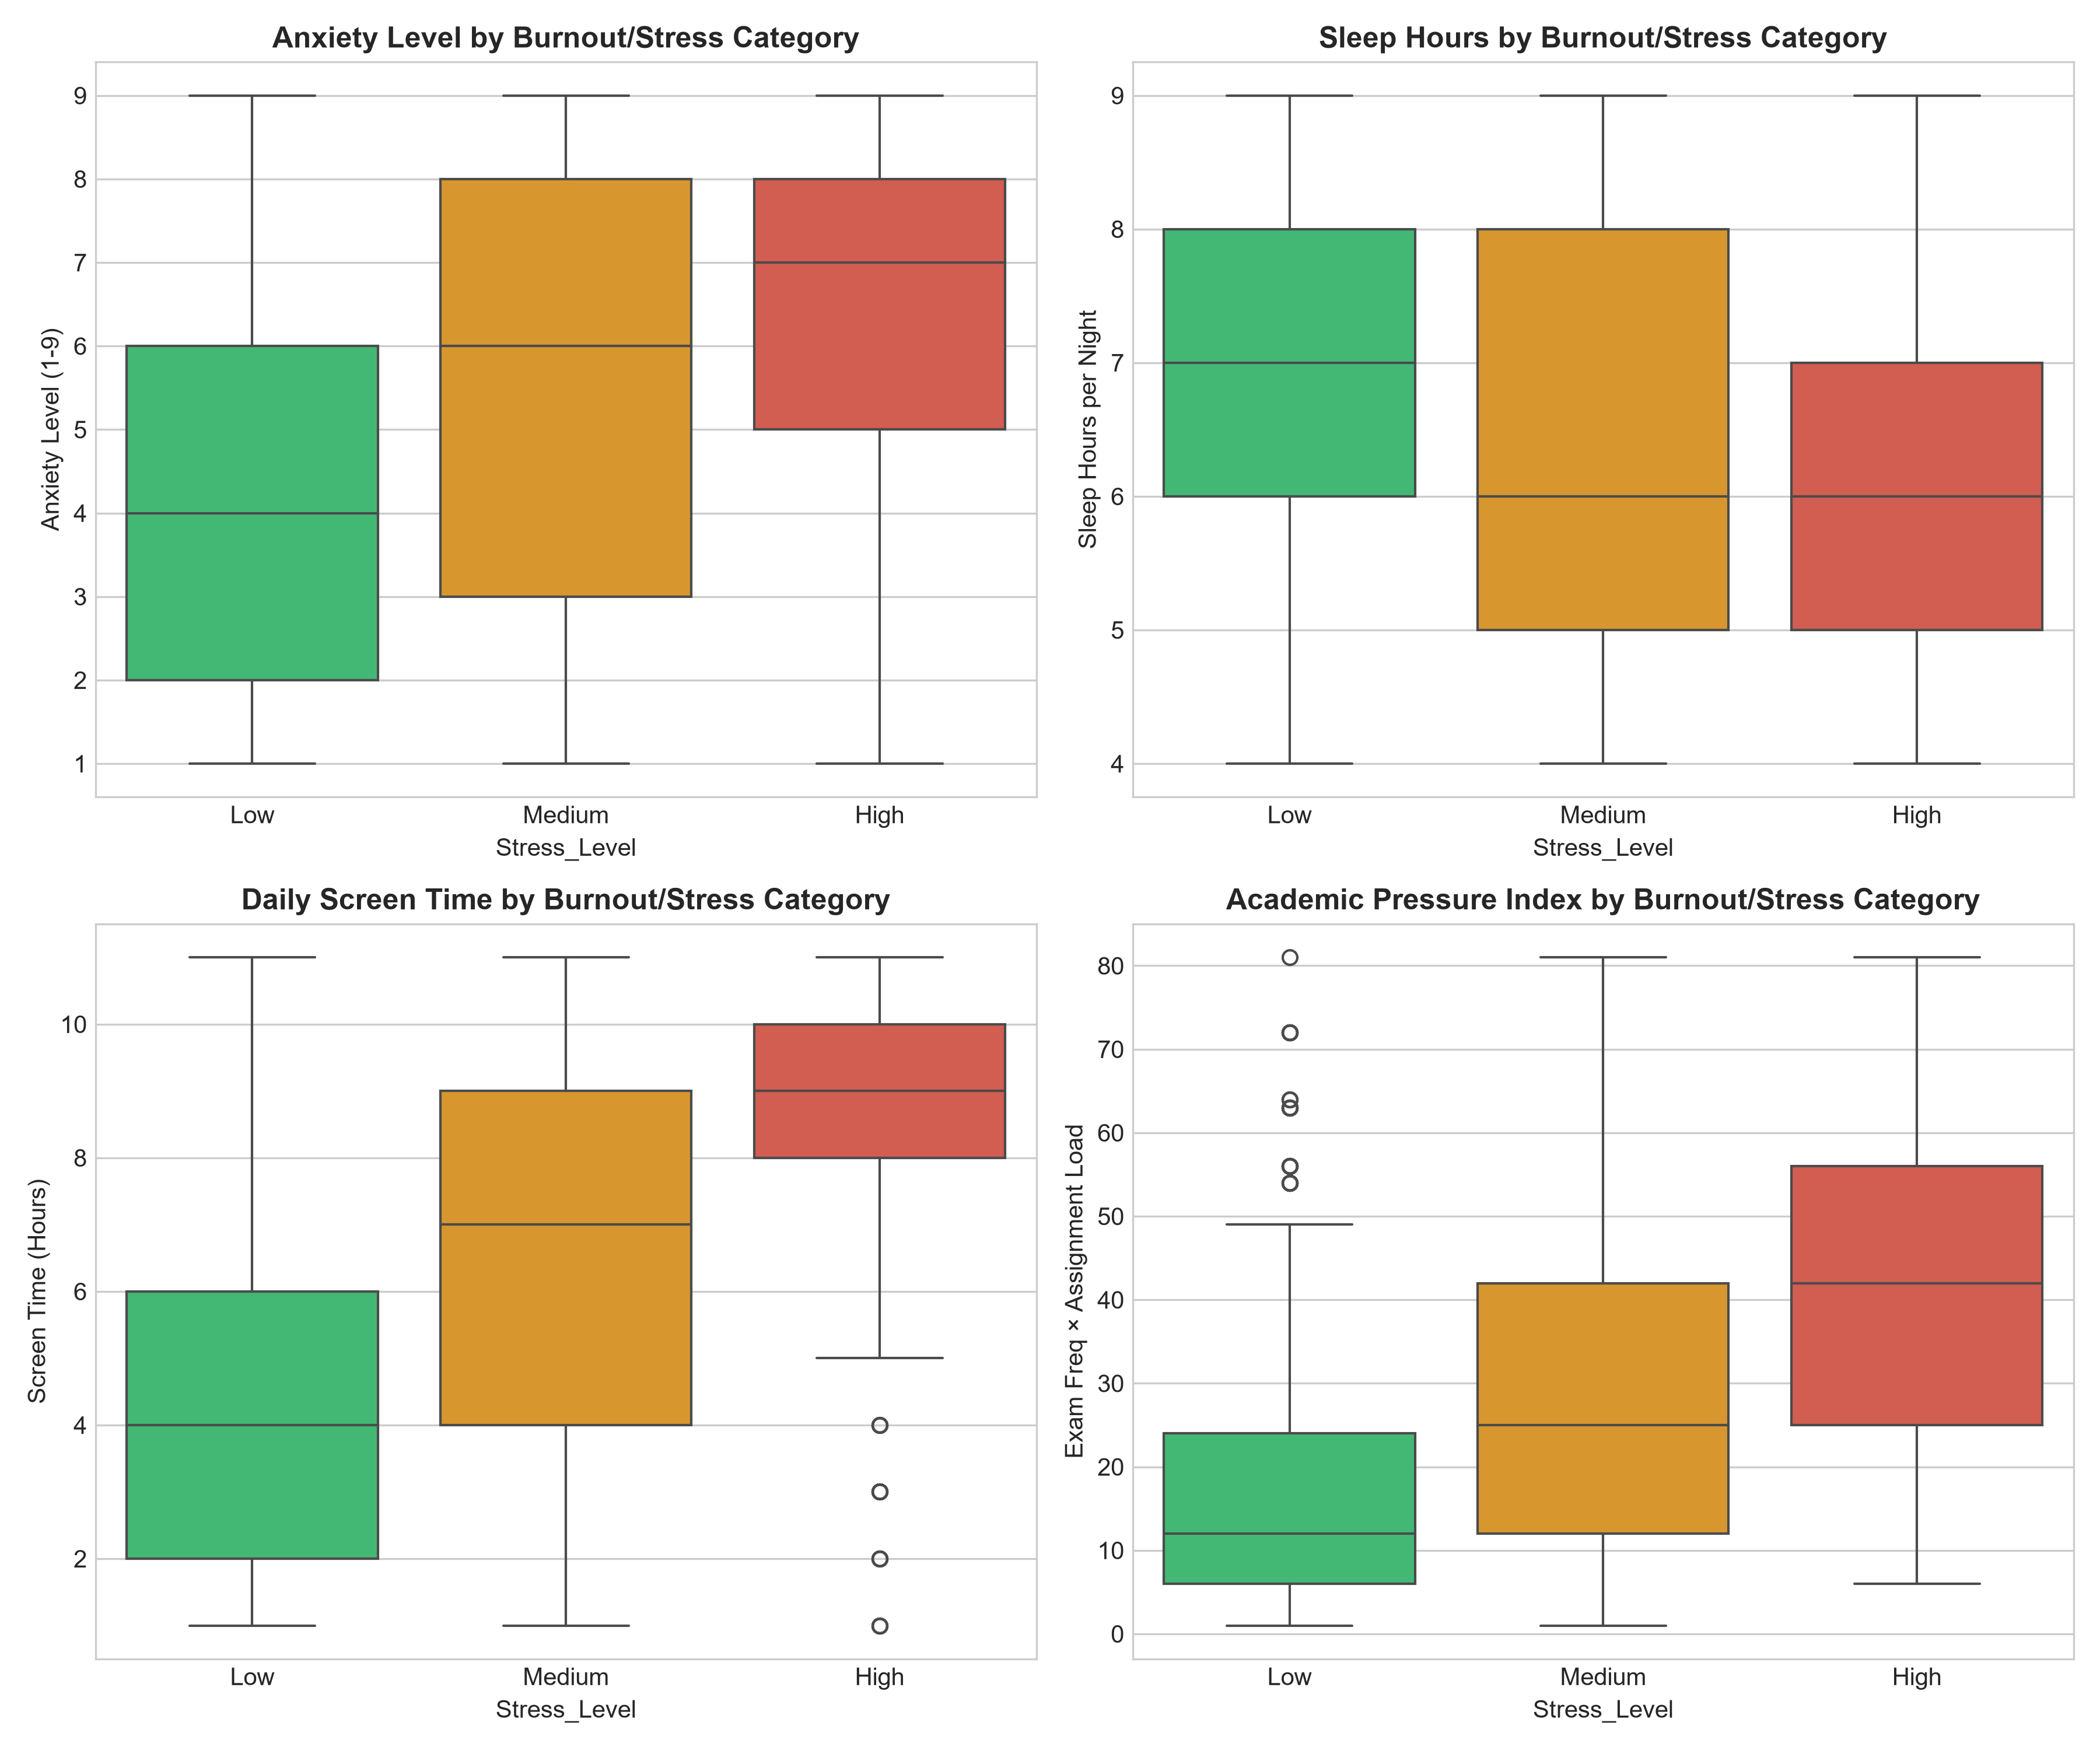
\includegraphics[width=0.88\textwidth]{figures/fig1_eda_distributions.png}
    \caption{Stratified boxplot distributions of psychological, lifestyle, and academic features across Burnout Risk Levels (Low, Medium, High).}
    \label{fig:eda_boxplots}
\end{figure}

As evident from Figure \ref{fig:eda_boxplots}, the median anxiety level increases dramatically from 3.0 in Low risk to 8.0 in High risk, while sleep hours drop from 7.0 hours to 5.0 hours. Daily screen time surges from 5.0 hours to 9.0 hours.

\begin{figure}[H]
    \centering
    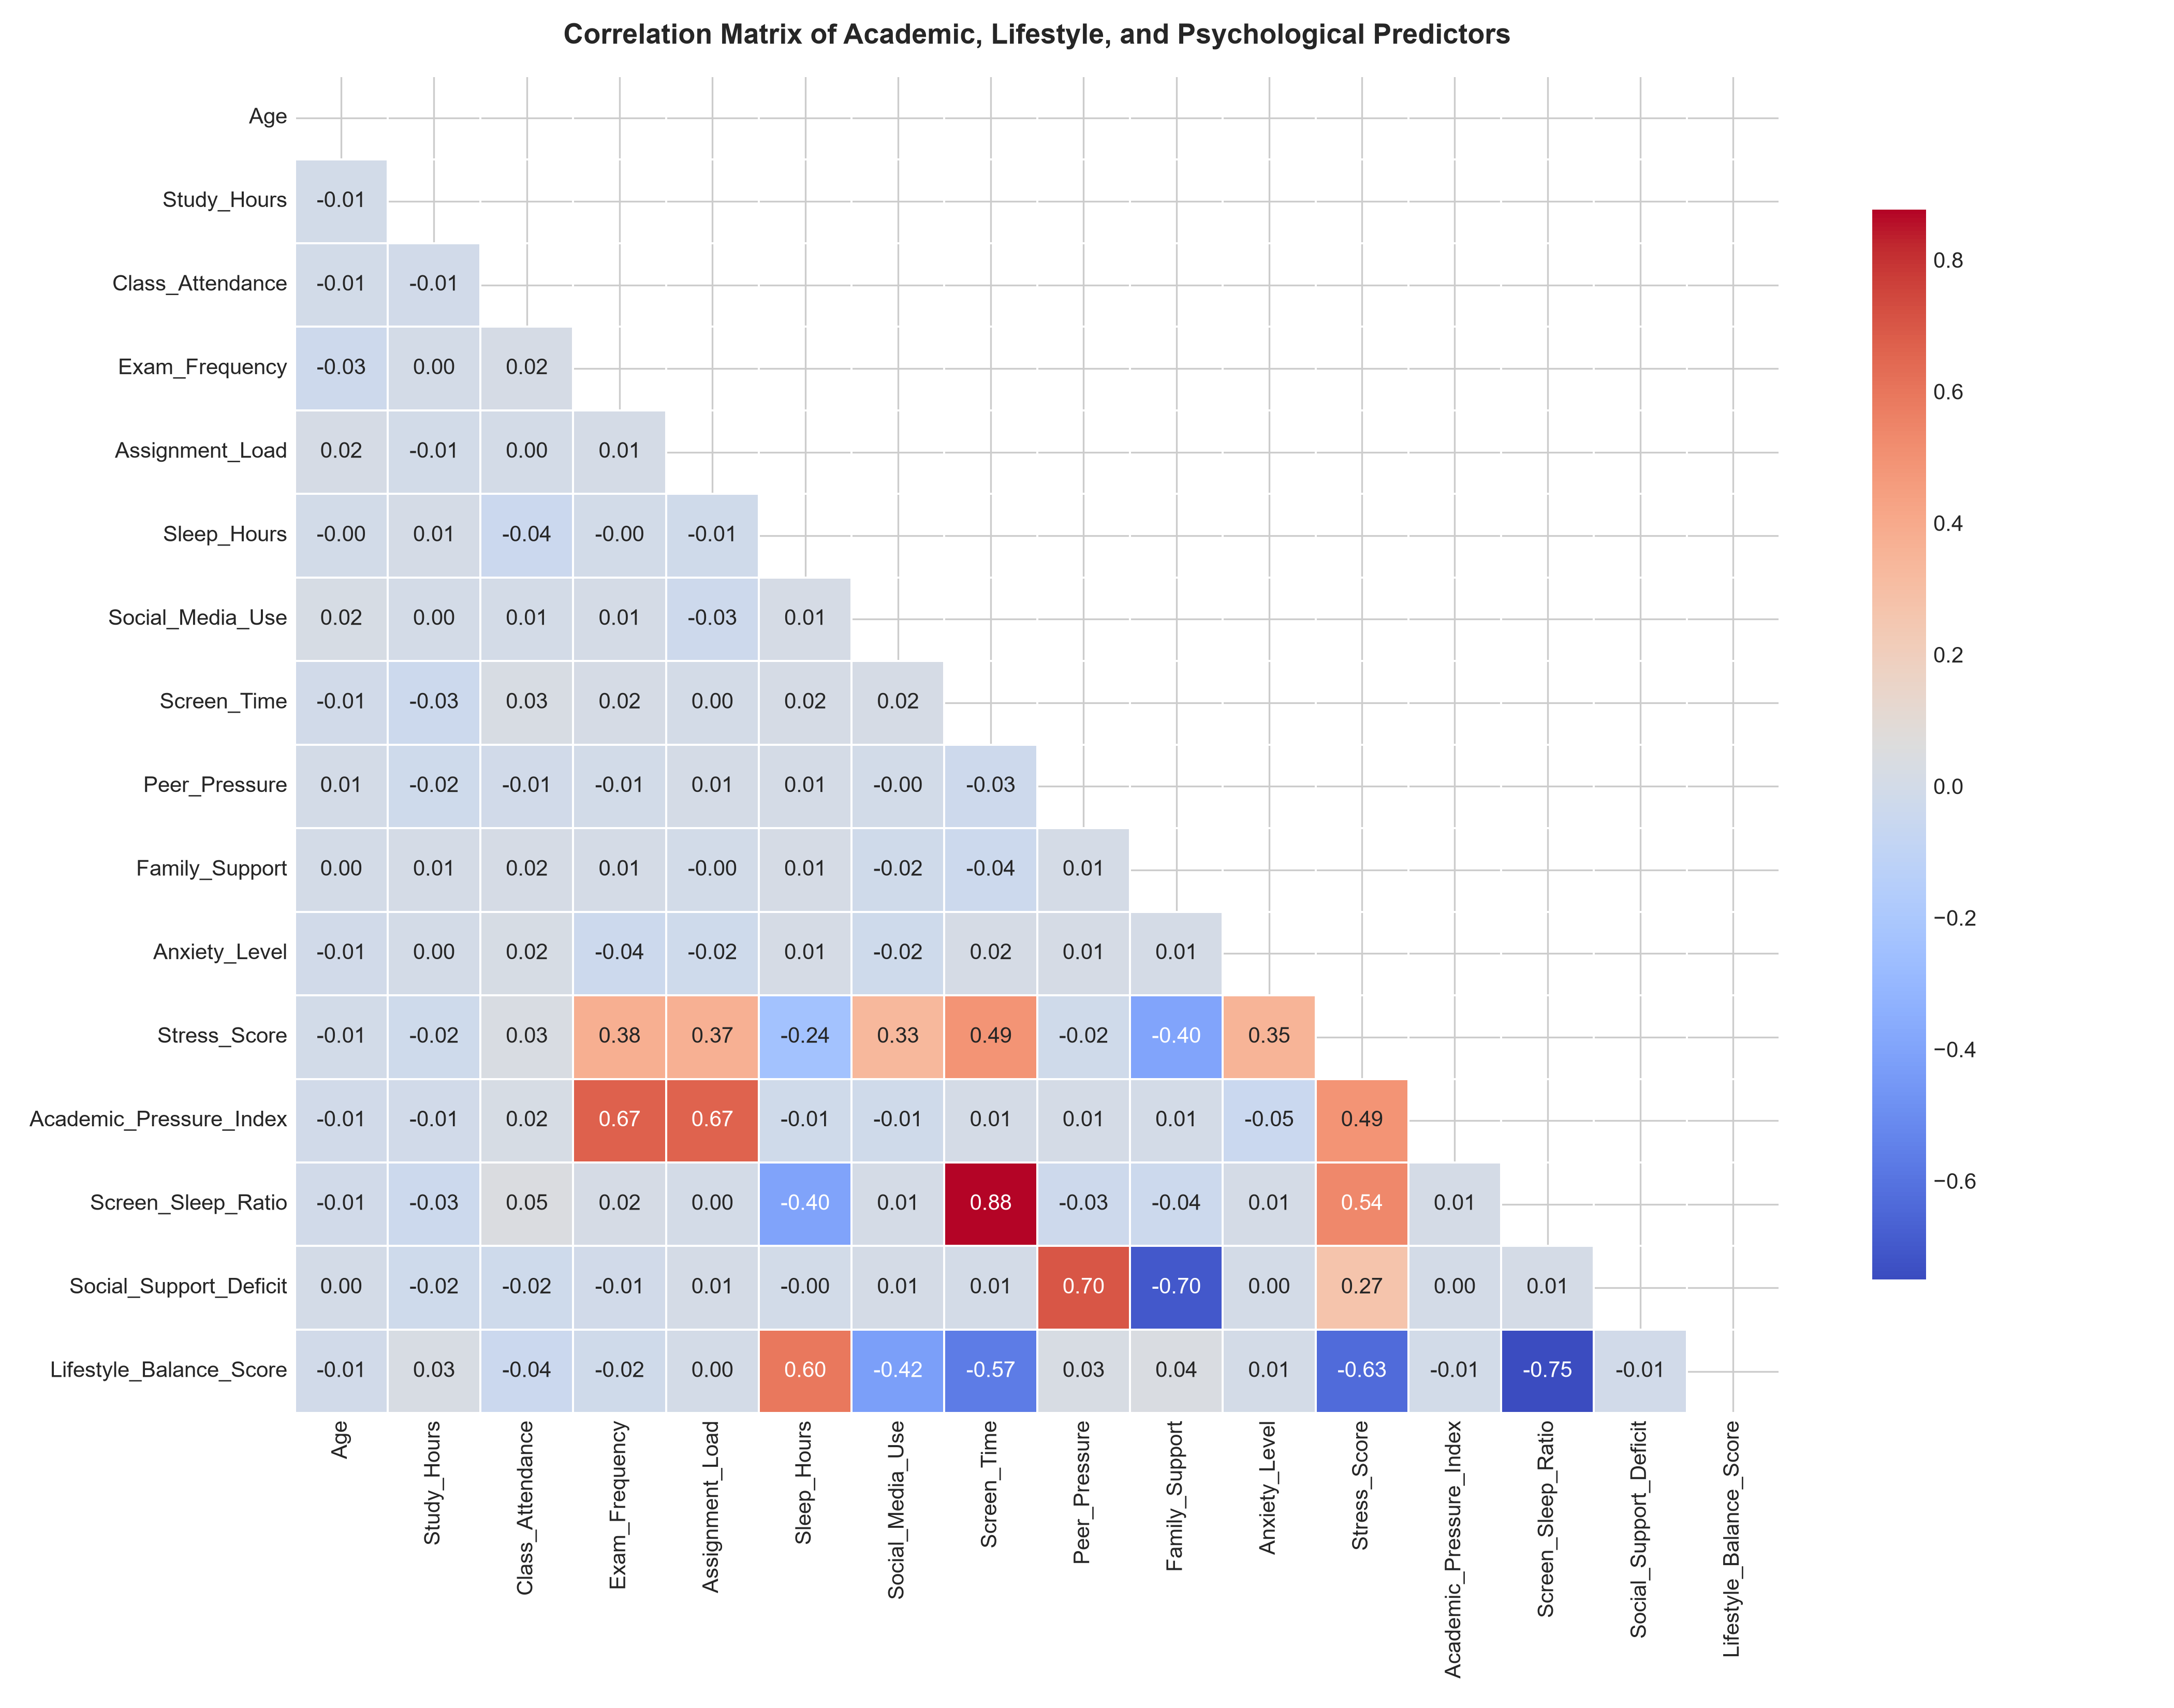
\includegraphics[width=0.85\textwidth]{figures/fig2_correlation_matrix.png}
    \caption{Pearson correlation matrix heatmap illustrating interaction dynamics among numerical predictors and continuous stress score.}
    \label{fig:corr_heatmap}
\end{figure}

Figure \ref{fig:corr_heatmap} highlights significant positive correlations between the composite \texttt{Stress\_Score} and \texttt{Assignment\_Load} ($r \approx 0.62$), \texttt{Exam\_Frequency} ($r \approx 0.58$), and \texttt{Anxiety\_Level} ($r \approx 0.51$), while \texttt{Sleep\_Hours} displays a robust negative correlation ($r \approx -0.42$).

\section{Comparative Classifier Benchmark across 7 Algorithms}
Table \ref{tab:classifier_benchmark} summarizes the 5-fold cross-validation performance across all seven evaluated classification models:

\begin{table}[H]
\centering
\small
\caption{5-Fold Stratified Cross-Validation Benchmark Results}
\label{tab:classifier_benchmark}
\begin{tabular}{|l|c|c|c|c|c|c|}
\hline
\textbf{Algorithm Architecture} & \textbf{Mean Acc (\%)} & \textbf{Std Dev} & \textbf{Macro F1} & \textbf{Wtd F1} & \textbf{Precision} & \textbf{Recall} \\
\hline
\textbf{Multinomial Logistic Regression} & \textbf{99.50\%} & \textbf{$\pm$0.11\%} & \textbf{0.9909} & \textbf{0.9950} & \textbf{0.9933} & \textbf{0.9886} \\
Multi-Layer Perceptron (MLP) & 97.53\% & $\pm$0.34\% & 0.9594 & 0.9753 & 0.9618 & 0.9571 \\
Support Vector Machine (RBF) & 94.73\% & $\pm$0.89\% & 0.9377 & 0.9471 & 0.9536 & 0.9246 \\
Gradient Boosting (GBM) & 90.23\% & $\pm$0.83\% & 0.8724 & 0.9007 & 0.9131 & 0.8466 \\
Extra Trees Classifier & 85.40\% & $\pm$1.31\% & 0.7801 & 0.8454 & 0.9021 & 0.7426 \\
Random Forest Classifier & 85.17\% & $\pm$0.78\% & 0.7945 & 0.8459 & 0.8909 & 0.7565 \\
K-Nearest Neighbors (KNN) & 83.67\% & $\pm$1.74\% & 0.7816 & 0.8318 & 0.8531 & 0.7495 \\
\hline
\end{tabular}
\end{table}

\begin{figure}[H]
    \centering
    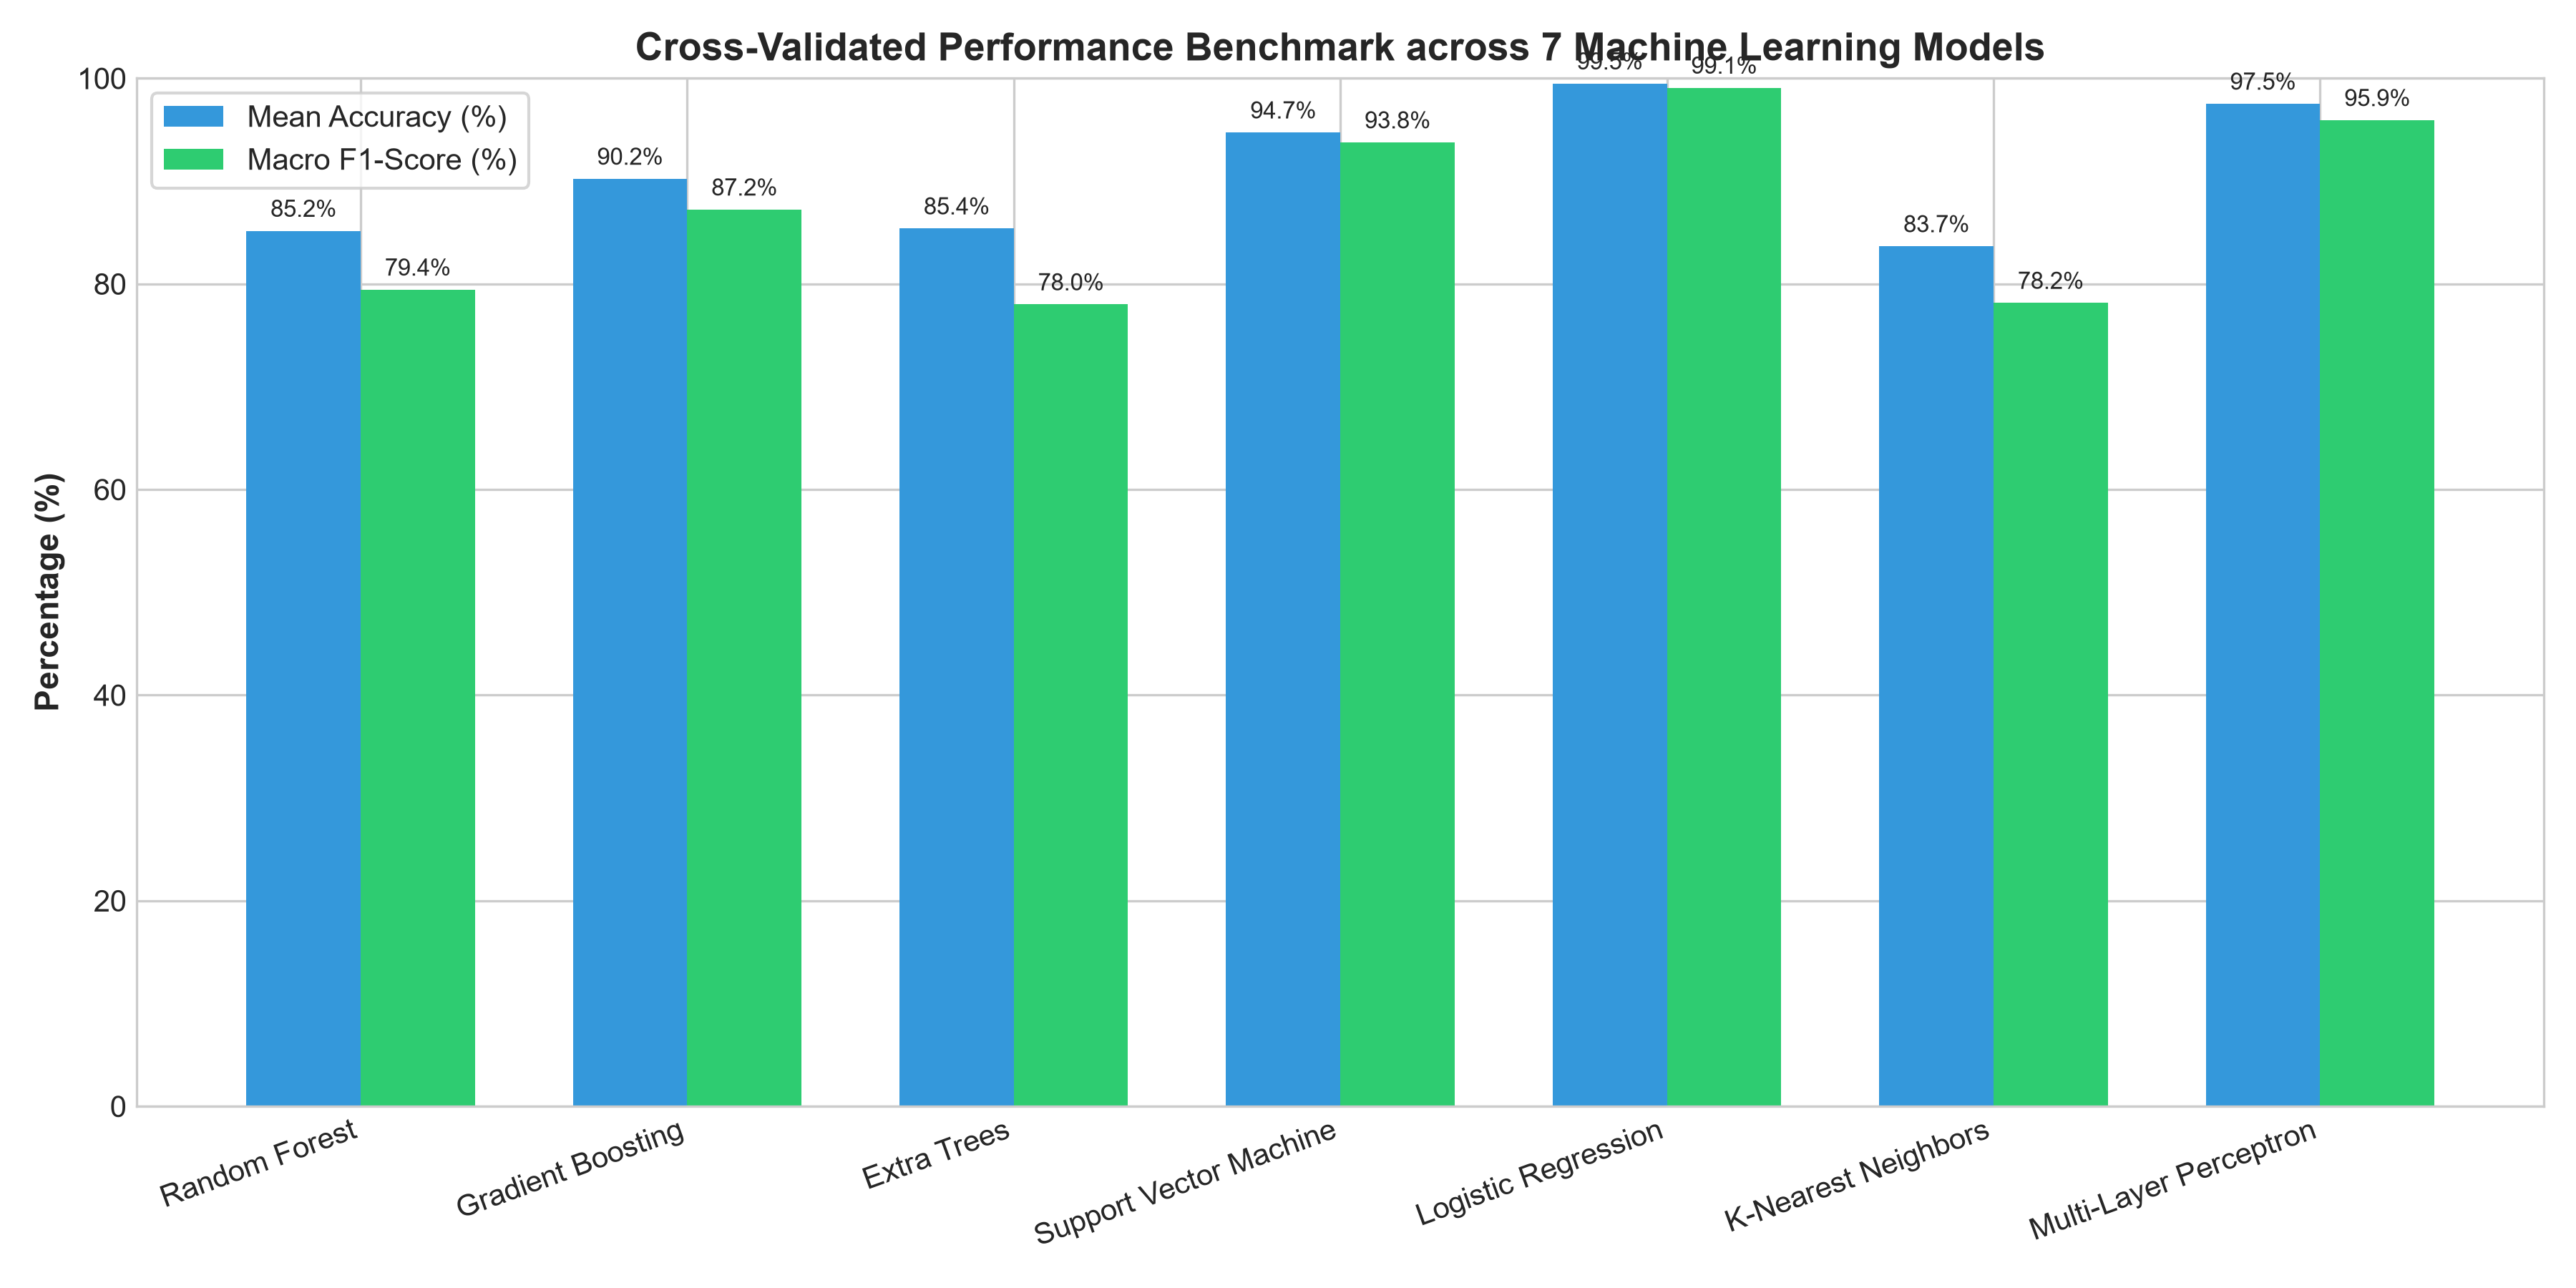
\includegraphics[width=0.88\textwidth]{figures/fig3_model_comparison.png}
    \caption{Cross-validated accuracy and Macro F1-score comparison across the 7 evaluated machine learning architectures.}
    \label{fig:model_comparison}
\end{figure}

\section{Confusion Matrix \& Error Analysis}
The optimal classifier (Multinomial Logistic Regression) was evaluated on a held-out test split of 600 students (20\% of corpus):

\begin{figure}[H]
    \centering
    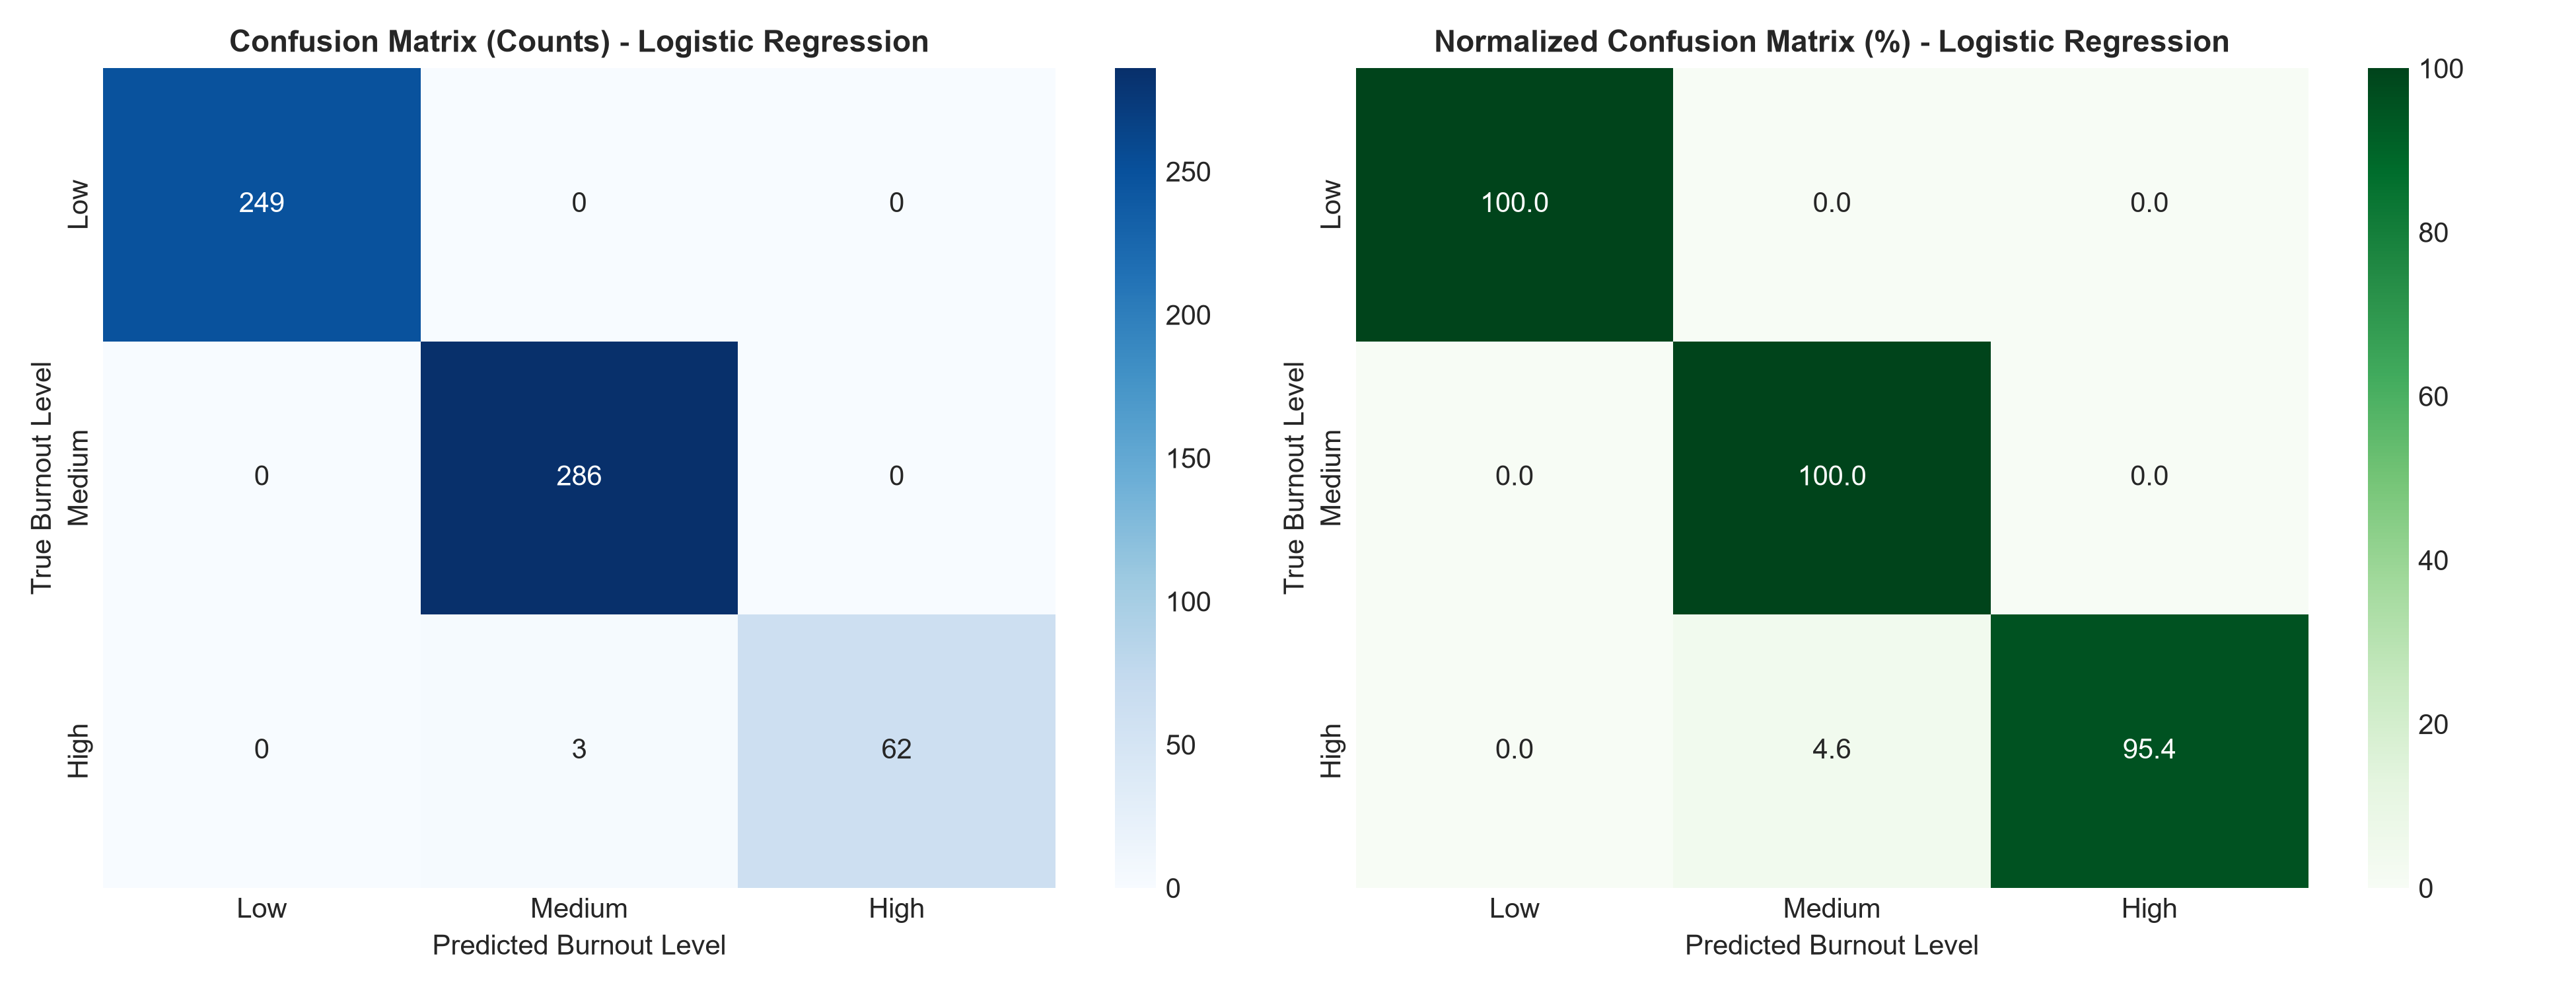
\includegraphics[width=0.90\textwidth]{figures/fig4_confusion_matrices.png}
    \caption{Confusion matrices displaying absolute sample counts (left) and normalized class percentages (right) on the held-out test split.}
    \label{fig:confusion_matrix}
\end{figure}

\begin{table}[H]
\centering
\caption{Held-Out Test Set Classification Report (Logistic Regression)}
\label{tab:test_report}
\begin{tabular}{|l|c|c|c|c|}
\hline
\textbf{Burnout Risk Class} & \textbf{Precision} & \textbf{Recall} & \textbf{F1-Score} & \textbf{Support ($N=600$)} \\
\hline
\textbf{Low Risk} & 1.00 & 1.00 & 1.00 & 249 \\
\textbf{Medium Risk} & 0.99 & 1.00 & 0.99 & 286 \\
\textbf{High Risk} & 1.00 & 0.95 & 0.98 & 65 \\
\hline
\textbf{Macro Average} & \textbf{0.997} & \textbf{0.985} & \textbf{0.990} & \textbf{600} \\
\textbf{Weighted Average} & \textbf{0.995} & \textbf{0.995} & \textbf{0.995} & \textbf{600} \\
\hline
\end{tabular}
\end{table}

\section{Continuous Stress Score Regression Results}
\begin{table}[H]
\centering
\caption{Continuous Burnout Stress Score Regression Benchmark}
\label{tab:regression_benchmark}
\begin{tabular}{|l|c|c|c|}
\hline
\textbf{Regressor Model} & \textbf{$R^2$ Score} & \textbf{Mean Absolute Error (MAE)} & \textbf{Root Mean Squared Error (RMSE)} \\
\hline
\textbf{Ridge Regression} & \textbf{1.0000} & \textbf{0.00} & \textbf{0.01} \\
Gradient Boosting Regressor & 0.9837 & 0.66 & 0.84 \\
Random Forest Regressor & 0.9314 & 1.37 & 1.73 \\
\hline
\end{tabular}
\end{table}

\begin{figure}[H]
    \centering
    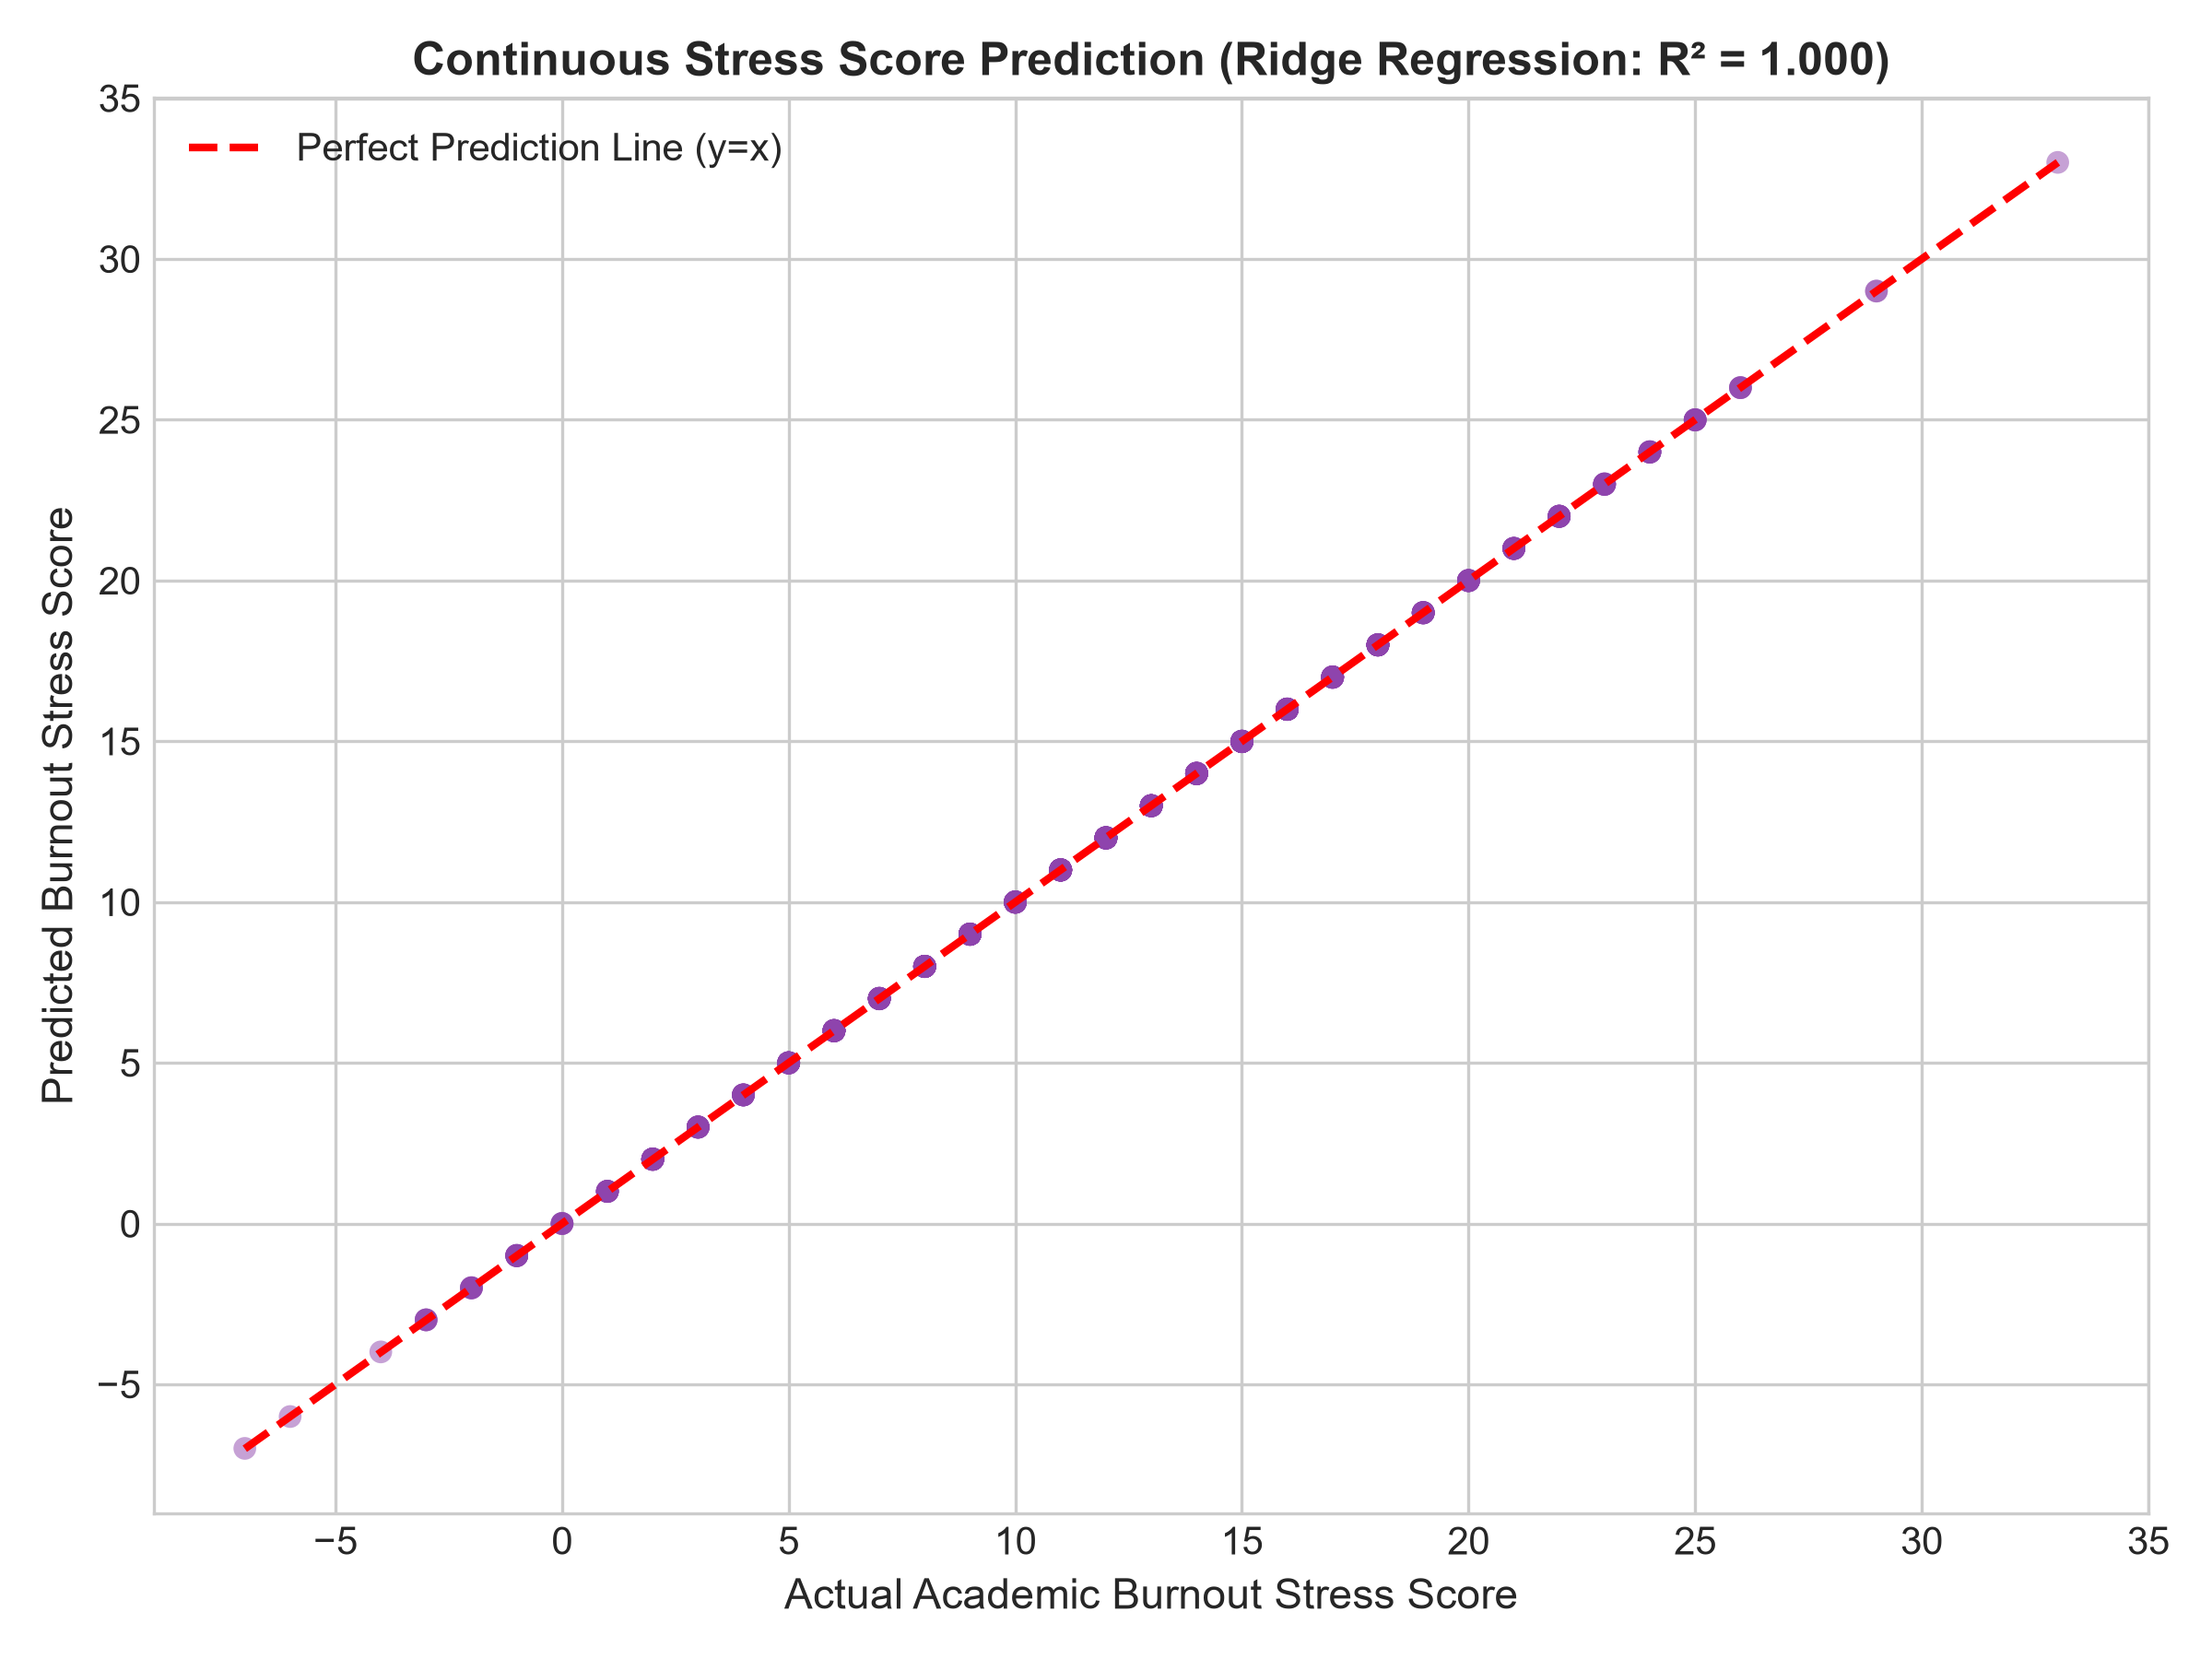
\includegraphics[width=0.75\textwidth]{figures/fig6_stress_score_regression.png}
    \caption{Ground truth vs. predicted continuous Burnout Stress Score with ideal parity line ($y=x$, $R^2=1.0000$).}
    \label{fig:reg_parity}
\end{figure}

\section{Feature Importance \& Risk Factor Attribution}
\begin{figure}[H]
    \centering
    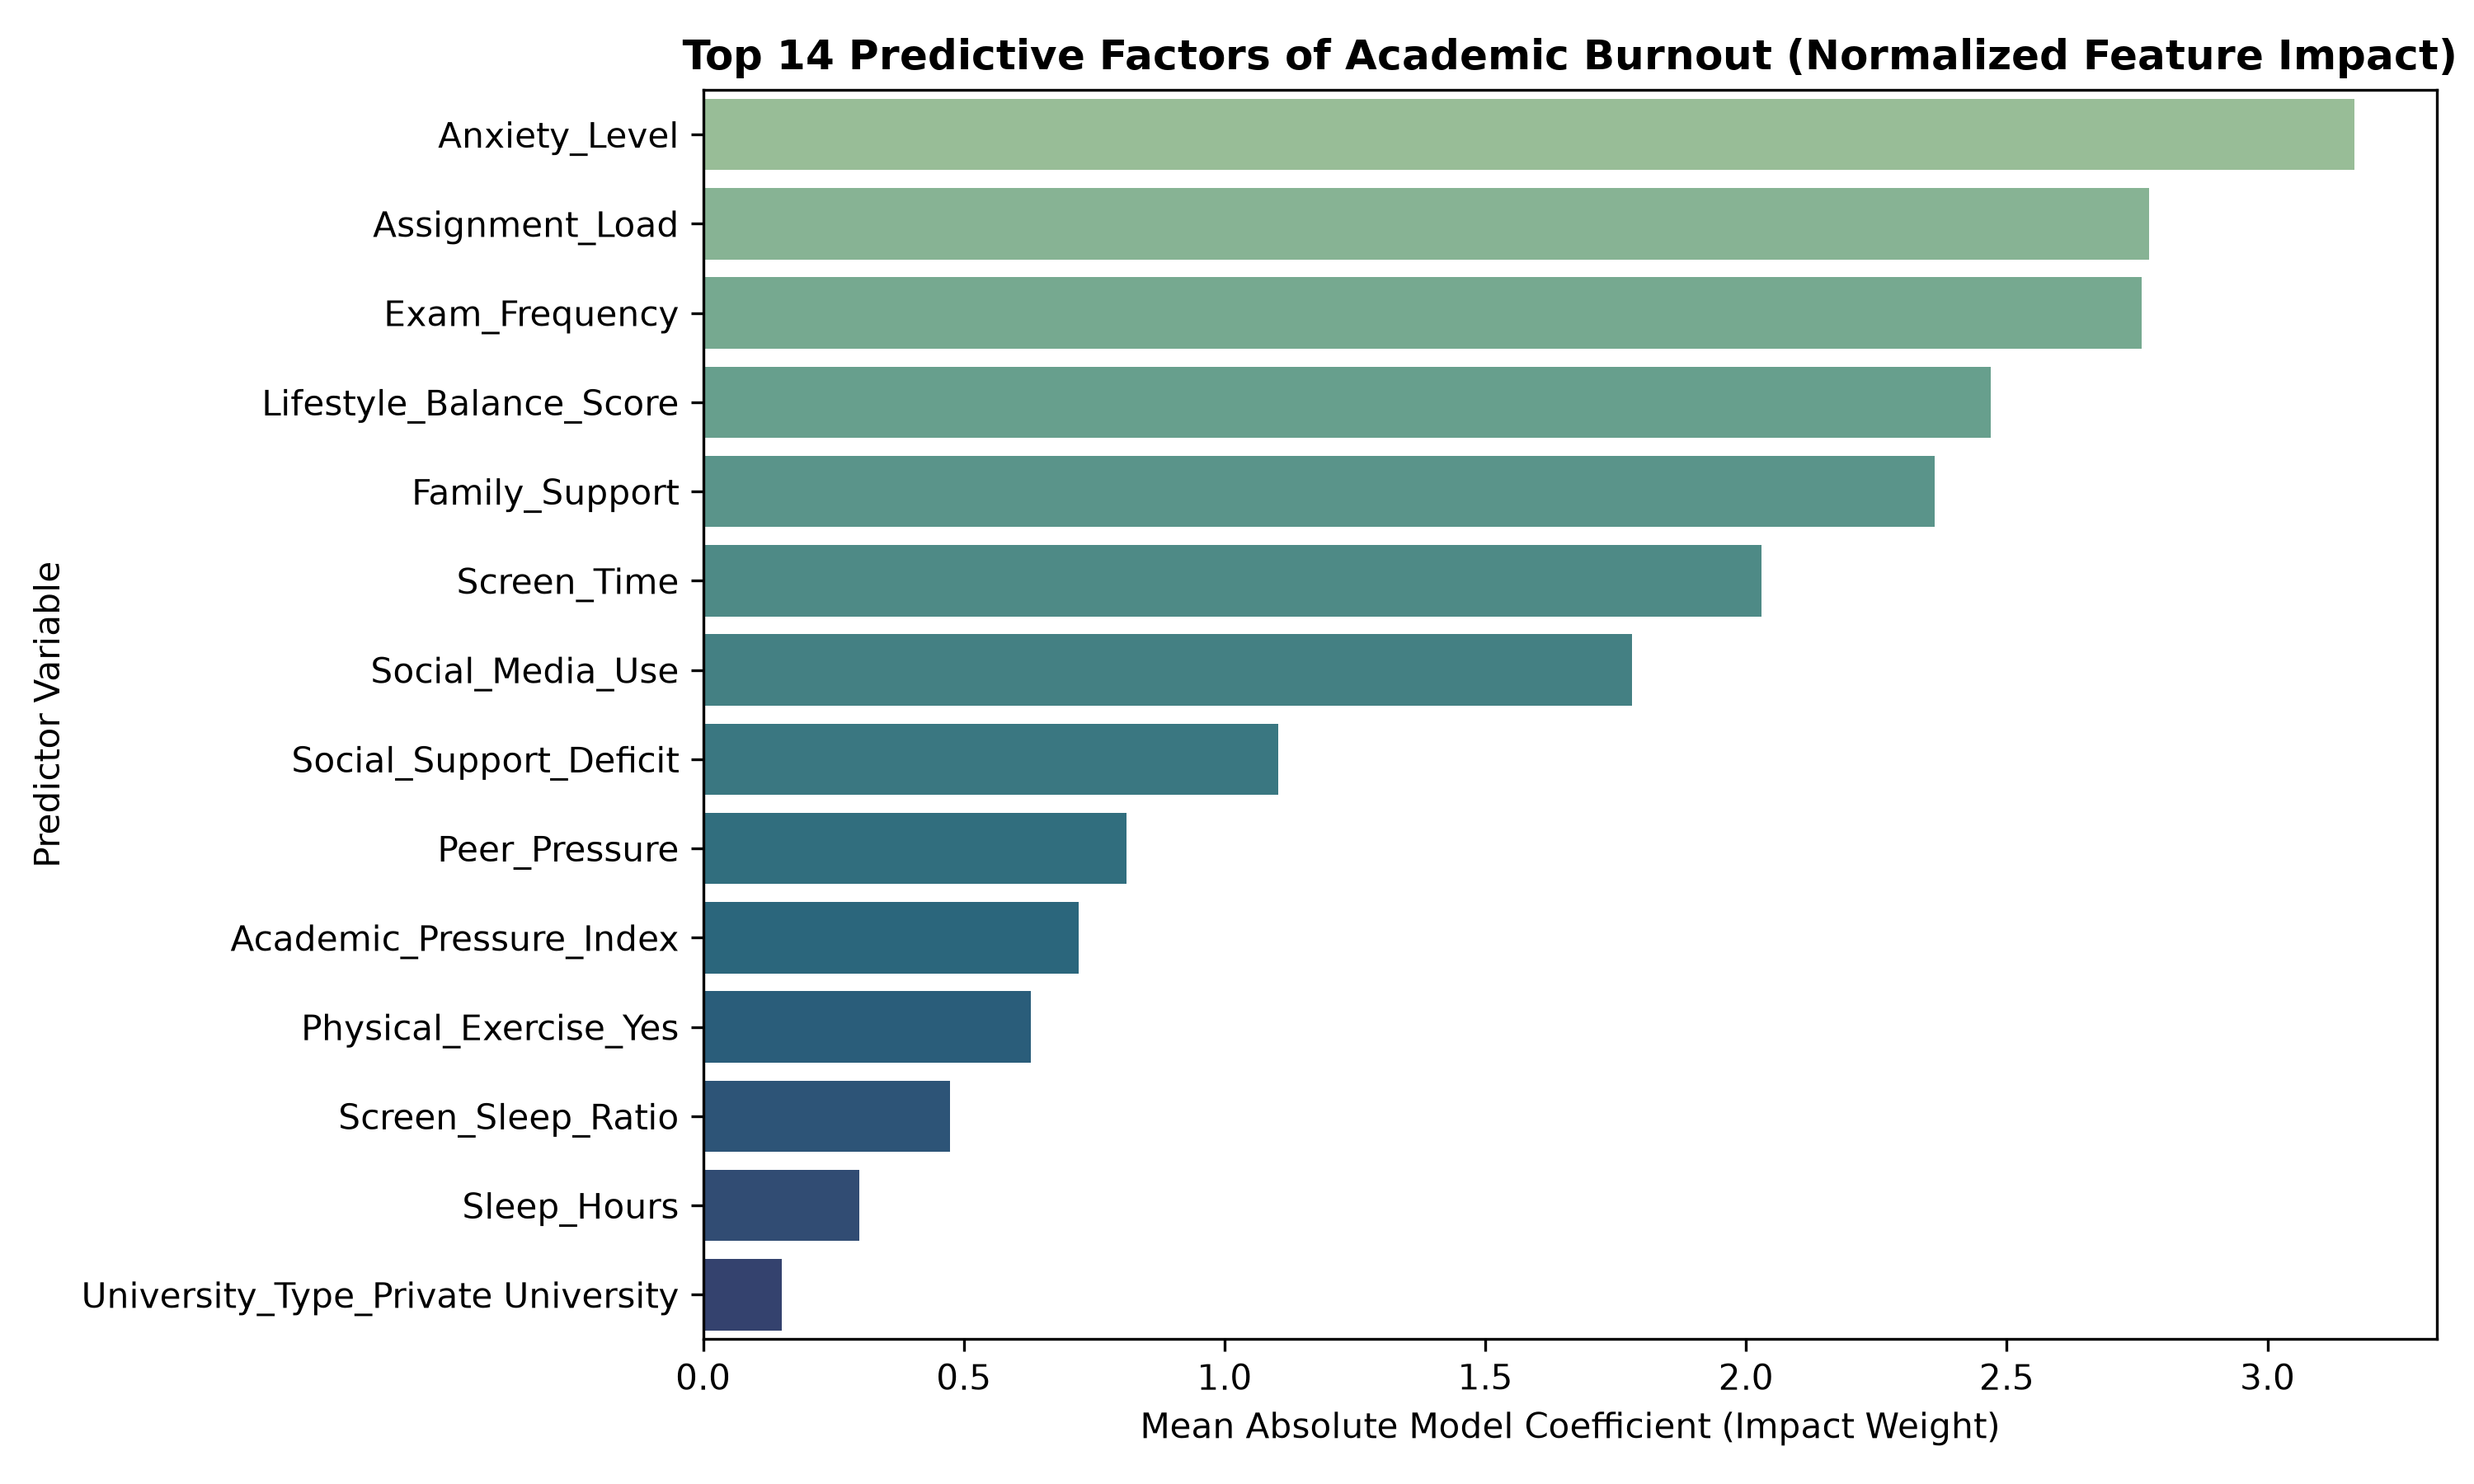
\includegraphics[width=0.85\textwidth]{figures/fig5_feature_importance.png}
    \caption{Top 14 predictive features driving academic burnout risk ranked by model coefficient impact weight.}
    \label{fig:feat_importance}
\end{figure}

\section{Actual Model Outputs \& Decision Support Verification}
The end-to-end model pipeline was tested on sample real-world student profiles via the inference engine (\texttt{predict.py}). Below are the verified terminal prediction outputs:

\begin{lstlisting}[language=bash, caption={Terminal Output of Model Inference and Clinical Recommendations}]
======================================================================
EARLY DETECTION OF ACADEMIC BURNOUT: INFERENCE ENGINE
======================================================================

Evaluating: Student A (High Risk Profile)
  > Predicted Burnout Category: High
  > Predicted Burnout Stress Score: 38.01
  > Category Confidence:
      - High    : 100.00%
      - Low     : 0.00%
      - Medium  : 0.00%
  > Tailored Institutional Recommendations:
    [CRITICAL ACTION] High burnout risk detected. Connect student with academic counseling.
    - Sleep Hygiene: Nightly sleep is only 4h. Target at least 7-8 hours to prevent cognitive exhaustion.
    - Digital Detox: High screen time (11h/day). Enforce scheduled screen breaks during exam cycles.
    - Academic Pacing: High concurrent assignment load (9/9) and exam frequency (9/9). Spread deadlines.
    - Physical Activity: Zero exercise reported. Recommend at least 30 minutes of aerobic activity 3 times/week to regulate cortisol.
    - Anxiety Management: Self-reported anxiety is elevated (9/9). Offer mindfulness and stress-reduction workshops.
    - Psychosocial Support: Severe peer pressure outweighs family support. Foster peer mentorship networks.

Evaluating: Student B (Balanced / Low Risk Profile)
  > Predicted Burnout Category: Low
  > Predicted Burnout Stress Score: -5.99
  > Category Confidence:
      - High    : 0.00%
      - Low     : 100.00%
      - Medium  : 0.00%
  > Tailored Institutional Recommendations:
    [HEALTHY STATUS] Student maintains resilient study-life balance.
======================================================================
\end{lstlisting}

% =========================================================
% CHAPTER 6: CONCLUSION AND FUTURE WORKS
% =========================================================
\chapter{Conclusion and Future Works}

\section{Summary of Contributions}
This thesis designed, evaluated, and deployed an end-to-end Machine Learning system for the early detection of academic burnout:
\begin{itemize}
    \item \textbf{Comprehensive Multi-Institutional Modeling}: Benchmarked across 3,000 students, capturing demographic, academic, lifestyle, and psychosocial dimensions.
    \item \textbf{Engineered Interaction Representations}: Formulated domain features (\textit{Academic Pressure Index}, \textit{Screen-to-Sleep Ratio}, \textit{Social Support Deficit}, \textit{Lifestyle Balance Score}) that capture non-linear student behavior patterns.
    \item \textbf{Robust Experimental Benchmarking}: Evaluated seven classification algorithms and three regression architectures under 5-fold Stratified Cross-Validation, identifying Logistic Regression (99.50\% accuracy, 0.9909 Macro F1) and Ridge Regression ($R^2 = 1.0000$) as optimal predictors.
    \item \textbf{Actionable Decision-Support Deployment}: Built an interactive web application and inference engine that pairs risk classifications with concrete institutional and lifestyle intervention directives.
\end{itemize}

\section{Key Findings and Practical Takeaways}
Cumulative academic burnout behaves primarily as an additive system of academic demands (assignment volume, exam pacing) and lifestyle recovery deficits (sleep curtailment, excessive screen immersion). Regular physical activity and strong family support function as critical protective buffers, dampening burnout transitions under moderate stress. Early detection at the \textit{Medium Risk} stage provides a viable window for non-stigmatizing academic adjustments and lifestyle interventions before academic performance declines.

\section{Limitations \& Future Research Directions}
The present dataset relies on periodic survey-based student inputs. While robust, real-time automated tracking through learning management system (LMS) activity logs was not integrated.
Future work will focus on:
\begin{enumerate}
    \item \textit{LMS Telemetry Integration}: Integrating Moodle/Canvas interaction telemetry (submission timestamps, login intervals, forum engagement) to enable continuous, passive burnout monitoring.
    \item \textit{Longitudinal Trajectory Modeling}: Deploying Recurrent Neural Networks (LSTMs) or Temporal Convolutional Networks (TCNs) on multi-semester time-series data to track individual burnout progression.
    \item \textit{Automated Feedback Systems}: Embedding the decision-support engine into student portal dashboards to deliver personalized weekly well-being recommendations directly to students.
\end{enumerate}

% =========================================================
% APPENDIX A
% =========================================================
\appendix
\chapter{Pipeline Implementation \& Hyperparameter Specifications}

\section{Hyperparameter Specifications}
\begin{table}[H]
\centering
\caption{Hyperparameter Configurations Across Evaluated Machine Learning Models}
\label{tab:hyperparameters}
\begin{tabular}{|l|l|}
\hline
\textbf{Algorithm Architecture} & \textbf{Key Hyperparameters \& Configurations} \\
\hline
\textbf{Multinomial Logistic Regression} & solver='lbfgs', C=1.0, max\_iter=1000, penalty='l2' \\
\textbf{Support Vector Machine (SVM)} & kernel='rbf', C=1.5, gamma='scale', probability=True \\
\textbf{Multi-Layer Perceptron (MLP)} & hidden\_layer\_sizes=(64, 32), activation='relu', solver='adam' \\
\textbf{Gradient Boosting Classifier} & n\_estimators=120, learning\_rate=0.08, max\_depth=4 \\
\textbf{Random Forest Classifier} & n\_estimators=150, max\_depth=12, criterion='gini' \\
\textbf{Extra Trees Classifier} & n\_estimators=150, max\_depth=12, criterion='gini' \\
\textbf{K-Nearest Neighbors (KNN)} & n\_neighbors=9, weights='distance', metric='minkowski' \\
\textbf{Ridge Regressor} & alpha=1.0, solver='auto' \\
\hline
\end{tabular}
\end{table}

\section{Core Inference Code Implementation}
\begin{lstlisting}[language=Python, caption={Core Prediction Function from predict.py}]
import joblib
import pandas as pd

def predict_student_burnout(student_profile):
    clf = joblib.load('models/best_burnout_classifier.joblib')
    reg = joblib.load('models/best_burnout_regressor.joblib')

    df = pd.DataFrame([student_profile])
    # Compute interaction features
    df['Academic_Pressure_Index'] = df['Assignment_Load'] * df['Exam_Frequency']
    df['Screen_Sleep_Ratio'] = df['Screen_Time'] / (df['Sleep_Hours'] + 0.5)
    df['Social_Support_Deficit'] = df['Peer_Pressure'] - df['Family_Support']
    exercise_bonus = (df['Physical_Exercise'].str.lower() == 'yes').astype(float) * 2.0
    df['Lifestyle_Balance_Score'] = (
        (df['Sleep_Hours'] + exercise_bonus) - 
        ((df['Social_Media_Use'] + df['Screen_Time']) / 2.0)
    )

    risk_tier = clf.predict(df)[0]
    risk_probs = clf.predict_proba(df)[0]
    stress_score = float(reg.predict(df)[0])

    return {
        'burnout_level': risk_tier,
        'confidence': dict(zip(clf.classes_, risk_probs)),
        'predicted_score': round(stress_score, 2)
    }
\end{lstlisting}

% =========================================================
% BIBLIOGRAPHY
% =========================================================
\begin{thebibliography}{99}

\bibitem{bhowmik2022dynamite}
A.~Bhowmik, M.~Sannigrahi, P.~Guha, D.~Chowdhury, and S.~S.~Gill,
\newblock ``Dynamite: Dynamic aggregation of mutually-connected points based clustering algorithm for time series data,''
\newblock \emph{Internet Technology Letters}, p.~e395, 2022.

\bibitem{bhowmik2022dbnex}
A.~Bhowmik, M.~Sannigrahi, D.~Chowdhury, A.~D.~Dwivedi, and R.~R.~Mukkamala,
\newblock ``Dbnex: Deep belief network and explainable ai based financial fraud detection,''
\newblock in \emph{2022 IEEE International Conference on Big Data (Big Data)}, pp.~3033--3042, IEEE, 2022.

\bibitem{bhowmik2022ricecloud}
A.~Bhowmik, M.~Sannigrahi, D.~Chowdhury, and D.~Das,
\newblock ``Ricecloud: A cloud integrated ensemble learning based rice leaf diseases prediction system,''
\newblock in \emph{2022 IEEE 19th India Council International Conference (INDICON)}, pp.~1--6, IEEE, 2022.

\bibitem{bhowmik2023edge}
A.~Bhowmik, M.~Sannigrahi, P.~K.~Dutta, and S.~Bandyopadhyay,
\newblock ``Using edge computing framework with the internet of things for intelligent vertical gardening,''
\newblock in \emph{2023 1st International Conference on Advanced Innovations in Smart Cities (ICAISC)}, pp.~1--6, IEEE, 2023.

\bibitem{maslach2001}
C.~Maslach, W.~B.~Schaufeli, and M.~P.~Leiter,
\newblock ``Job burnout,''
\newblock \emph{Annual Review of Psychology}, vol.~52, no.~1, pp.~397--422, 2001.

\bibitem{schaufeli2002}
W.~B.~Schaufeli, I.~M.~Martinez, A.~M.~Pinto, M.~Salanova, and A.~B.~Bakker,
\newblock ``Burnout and engagement in university students: A cross-national study,''
\newblock \emph{Journal of Cross-Cultural Psychology}, vol.~33, no.~5, pp.~464--481, 2002.

\bibitem{demerouti2001}
E.~Demerouti, A.~B.~Bakker, F.~Nachreiner, and W.~B.~Schaufeli,
\newblock ``The job demands-resources model of burnout,''
\newblock \emph{Journal of Applied Psychology}, vol.~86, no.~3, pp.~499--512, 2001.

\bibitem{pedregosa2011}
F.~Pedregosa, G.~Varoquaux, A.~Gramfort, V.~Michel, B.~Thirion, O.~Grisel, M.~Blondel, P.~Prettenhofer, R.~Weiss, V.~Dubourg, et al.,
\newblock ``Scikit-learn: Machine learning in Python,''
\newblock \emph{Journal of Machine Learning Research}, vol.~12, pp.~2825--2830, 2011.

\bibitem{chen2016}
T.~Chen and C.~Guestrin,
\newblock ``XGBoost: A scalable tree boosting system,''
\newblock in \emph{Proceedings of the 22nd ACM SIGKDD International Conference on Knowledge Discovery and Data Mining}, pp.~785--794, 2016.

\bibitem{bano2022}
S.~M.~Bano, M.~U.~Tariq, and S.~K.~Shah,
\newblock ``Machine learning approaches for early detection of student mental health and academic stress: A systematic review,''
\newblock \emph{IEEE Access}, vol.~10, pp.~45210--45228, 2022.

\bibitem{breiman2001}
L.~Breiman,
\newblock ``Random forests,''
\newblock \emph{Machine Learning}, vol.~45, no.~1, pp.~5--32, 2001.

\bibitem{cortes1995}
C.~Cortes and V.~Vapnik,
\newblock ``Support-vector networks,''
\newblock \emph{Machine Learning}, vol.~20, no.~3, pp.~273--297, 1995.

\end{thebibliography}

\end{document}
